% !TeX program = lualatex
% Compile twice with LuaLaTeX so the table of contents resolves.
\documentclass[11pt]{article}
\usepackage[a4paper,margin=24mm]{geometry}
\usepackage{fontspec}
\defaultfontfeatures{Ligatures=TeX}
\setmainfont{Latin Modern Roman}
\setsansfont{Latin Modern Sans}
\setmonofont{Latin Modern Mono}
\usepackage{microtype}
\usepackage{amsmath,amssymb}
\usepackage{booktabs,longtable,array}
\usepackage{enumitem}
\usepackage{xcolor}
\usepackage{hyperref}
\usepackage{caption}
\usepackage{fvextra}
\usepackage{tikz}
\usepackage{pgfplots}
\pgfplotsset{compat=1.18}
\hypersetup{colorlinks=true,linkcolor=blue!50!black,urlcolor=blue!60!black,citecolor=blue!50!black,pdftitle={Fly-Brain Circuits for a Personal AI Agent},pdfauthor={The Aiko-chan Project Contributors}}
\setlength{\parindent}{0pt}
\setlength{\parskip}{.55em}
\setlength{\tabcolsep}{2pt}
\setcounter{tocdepth}{2}
\DefineVerbatimEnvironment{CodeBlock}{Verbatim}{breaklines=true,breakanywhere=true,fontsize=\small,frame=single,framesep=3mm,rulecolor=\color{black!20}}
\newcommand{\tightsection}{\vspace{-.25em}}
\title{Fly-Brain Circuits for a Personal AI Agent:\\ Modulatory Neuromorphic Subsystems Around an LLM Core}
\author{The Aiko-chan Project Contributors\\\small Independent research · OppaAI, Canada}
\date{30 September 2026}
\begin{document}
\maketitle
\begin{abstract}
We describe Aiko-chan's fly-brain stack, a set of connectome-inspired control and learning circuits built around a large language model (LLM). The system does not replace language understanding or planning. It supplies fast, bounded signals for learned value, orientation, salience, interruption, motor vigor, delayed credit, persona-conditioned bias, and deployment observability. A per-user registry prevents state cross-talk, while a shared \texttt{NeuralState} record provides one inspectable read model for the agent loop.

The implementation developed in two layers. Stages 0-6.1 connected mushroom body, central complex, antennal/lateral-horn, T4/T5 motion, giant-fiber, and descending-neuron motifs to Aiko's memory, ReAct loop, speech, body packet, and VRM companion. A subsequent twelve-phase engineering program hardened the runtime: process guards; batching and deduplication; quiet headless operation; full MaleCNS propagation; action selection; sensory pathways; persistent central-complex dynamics; replay; a closed-loop practice world; rate-based dopamine and eligibility traces; motor coordination; bounded persona modulation; and metrics with safe manual dialing.

Representative implemented equations include a blended fly/LLM action score with fly weight \(\lambda=0.25\), a giant-fiber veto at valence \(-0.6\), bounded central-complex state updates, and the Phase 10A learning chain: \(E\leftarrow\operatorname{clip}(E+0.2(r-E),-1,1)\), \(e\leftarrow e\,0.5^{1/6}\), and \(\Delta w=\operatorname{clip}(d_a e\,LR,-1,1)\), with a 1.6 reversal multiplier. Phase 12 adds \texttt{applied\_rate}, \texttt{agree\_rate}, \texttt{fullbrain\_avg\_ms}, and a dual turn/time throttle; it deliberately adds neither spiking neurons nor automatic weight tuning.

\medskip\noindent \textbf{Keywords:} Drosophila-inspired circuits, modulatory control, MaleCNS, action selection, eligibility traces, shadow deployment, personal agents
\end{abstract}
\tableofcontents
\clearpage

\section{Introduction}

A fruit fly flies with roughly \(10^5\) neurons and a body it owns for weeks, making thousands of fine-grained decisions per second in real time on milliwatts of energy. A personal AI agent runs on a thermals-and-RAM-limited single board computer — in our case an NVIDIA Jetson — facing the same shape of problem: watch the world, decide what matters, gate effort, remember what worked, and stay safe while doing it. Our thesis is that \emph{Drosophila} circuit motifs — fast sensors, bounded integrators, competitive voting, eligibility-trace learning — are a good architectural vocabulary for the non-linguistic half of an agent, and that they can coexist with a language model rather than compete with it.

The fly-brain stack developed over twelve numbered phases. It is deliberately \emph{not} a world model, not a planner, and not a replacement for the LLM. It is a set of \emph{modulatory subsystems}: small circuits whose outputs weight, gate, or (in one carefully limited case) veto candidate actions. The LLM proposes and explains; the fly votes and gates; a Studio metric layer (Phase 12) records what happened so humans can tune the few knobs deliberately rather than by guesswork.

\begin{quote}
Reading guide: §2 states the two non-negotiable principles (shadow-first deployment; modulatory-only authority). §3 walks the integration history — Stages 0–6.1, the grafts and hardening the formal program rebuilt. §4–§8 walk the twelve phases with the shipped formulas; §8 includes measured-structure charts and an interactive throttle simulator built from the same data set. Readers who only care about operating the system can read §8 alone.
\end{quote}
\section{Design principles}

\subsection{Shadow-first, per-phase, fully reversible}

Behavior-bearing circuit layers use narrow configuration gates, normally \texttt{off}, \texttt{shadow}, or \texttt{live}. In shadow mode the layer computes and logs but does not steer behavior; in live mode the same output is allowed to bias the next downstream decision. Infrastructure phases use ordinary bounded settings instead: Phase 1 has a lock timeout, Phase 2 controls deduplication and batching, and Phase 3 retimes background services. This distinction avoids pretending that a process guard or a database flush has a meaningful "shadow" state.

Reversibility remains local. \texttt{AIKO\_FLY\_ACTION\_MODE}, \texttt{AIKO\_FLY\_SENSE\_MODE}, \texttt{AIKO\_FLY\_CX\_MODE}, \texttt{AIKO\_FLY\_REPLAY\_MODE}, \texttt{AIKO\_FLYWORLD\_MODE}, \texttt{AIKO\_FLY\_DOPAMINE\_MODE}, \texttt{AIKO\_FLY\_BODY\_MODE}, and \texttt{AIKO\_FLY\_PERSONA\_MODE} can be changed independently. The active connectome service adds \texttt{AIKO\_FLY\_RUNTIME\_MODE}, defaulting to \texttt{off}. A bad observation can therefore retreat one layer from live to shadow without deleting learned state or disabling the LLM.

\subsection{Modulatory subsystems, never a replacement}

The LLM core owns language understanding, tool use, and deliberation. The fly circuits own the non-linguistic surround: urgency, heading, effort cost, learned value, veto reflexes. The interfaces between them are narrow:

\begin{enumerate}[leftmargin=*]
\item \textbf{Propose.} The LLM (and classical schedulers) propose candidate actions.
\item \textbf{Vote.} The Phase 5 action vote scores candidates by circuit consensus, keeping the argmax but blending with LLM scores at \(\lambda = 0.25\).
\item \textbf{Gate.} Effort (Phase 2), urgency (Phase 7), and trace-learned value (Phase 10A) scale scores or impose costs before anything executes.
\item \textbf{Veto.} Only the giant-fiber escape channel may hard-block an action, and only when valence clears a loud threshold (§4.5).
\end{enumerate}

Consequence: no circuit can initiate an act on its own. If every circuit is switched \texttt{off}, the agent is a plain LLM agent — slower reflexes, but correct core behavior. The stack can only make it faster, more consistent, and more self-aware, proportional to how far each dial is turned up.

\subsection{The reference model is an offline artifact}

Two MaleCNS representations coexist and must not be confused. Phase 4 introduced a process-wide, rate-based full graph over 166,606 neurons and 25,574,615 directed edges, stored as a compact NPZ and propagated for two hops from mushroom-body Kenyon-cell seeds. The later active runtime uses a \texttt{ConnectomeCatalog} built from the MaleCNS v1.0 minconf-0.5 release: 211,577 catalog nodes and 6,300,108 retained edges at weight at least 5. The catalog verifies its declared SHA-256 digest and answers only bounded subgraph queries.

Both are engineering abstractions informed by anatomy. The graph edges and transmitter signs come from the source data; the rate update, seed injection, readout groups, node budgets, and behavioral interpretation are synthetic. This boundary is explicit in code and matters scientifically: the implementation is connectome-constrained, not a claim to simulate a biological fly.

\section{Stages 0–6.1: connecting the fly brain to Aiko}

Before the numbered phases were a program, they were a graft. On 18 September 2026 the first MaleCNS wiring was merged into Aiko-chan: modules named for fly circuitry — a mushroom-body model reading value, a compass carrying heading, descending-neuron channels carrying readiness — woven into a living agent a user talks to every day. Over that September the wiring went from thin demonstration grafts to the working stack: a hardening migration that tore out shared process-wide state, an active MaleCNS runtime verified against a shipped connectome dataset, and then seven integration stages, each wiring a fly circuit into a concrete agent capability instead of leaving it a promising module in a directory. The record lives in the repository docs: \texttt{docs/FLY\_STAGE1.md} through \texttt{docs/FLY\_STAGE6\_1.md}, \texttt{docs/FLY\_BRAIN\_WIRING.md}, \texttt{docs/FLY\_BRAIN\_ROADMAP.md}, \texttt{docs/FLY\_ACTIVE\_RUNTIME.md}, and \texttt{docs/FLY\_COMPLETE.md}.

This section walks that integration history with the code shapes it produced. A reader who wants just the formal program can skip straight to §4 — but it helps to know where the contracts came from. The numbered \textbf{Phases 2–12} of §4–§8 are the formal optimization-program rebuild \emph{on top of this groundwork}: every phase took a stage integration and re-derived it as an engineered, shadow-first, bounded, reversible contract. The stages are the archaeology; the phases are the architecture that the archaeology justified.

\subsection{Stage 0 — first grafts and the hardening migration}

The 2026-09-18 grafts landed in the shape every prototype starts in: module-level singletons. One \texttt{FlyMB} mushroom body and one \texttt{FlyCompass} compass per \emph{process}, shared by every user, every session, every conversation. In a demo that is fine; in a personal agent where one handler may juggle contexts — and where fly state \emph{remembers} — it is a correctness defect: anything user A teaches the fly leaks straight into user B's reads.

The hardening migration replaced that shape with \texttt{cognition.fly\_registry}: a registry of per-user fly-state bundles, lazy-constructed and isolated. \textbf{User A → fly state A; user B → fly state B; no cross-talk.} The migration is before/after simple — every read path switches from a module global to a registry lookup keyed by user id:

\begin{CodeBlock}
# Stage 0 — BEFORE: module-level FlyMB/FlyCompass singletons (shared by everyone)
_mb = FlyMB()                       # one mushroom body per *process*
_compass = FlyCompass()             # one compass per process
                                    # what user A teaches leaks into user B's read
# Stage 0 — AFTER: cognition.fly_registry per-user isolation
from cognition import fly_registry

def fly_read(user_id, text):
    fly = fly_registry.get(user_id) # user A -> fly state A; user B -> fly state B
    return fly.mb.valence(text)     # reads can no longer see another user's state
\end{CodeBlock}

The migration's second invention outlives it: the \textbf{NeuralState bus} — the single read model of the whole fly. Instead of every consumer reaching into module internals, every module reports into one shared bus record, and every consumer reads from it:

\begin{CodeBlock}
# Stage 0 — NeuralState: the single read model for everything above the modules
from dataclasses import dataclass

@dataclass(frozen=True)
class NeuralState:                 # one bus record; all consumers read HERE
    valence: float                 # mushroom-body readout, [-1, 1]
    approach: float                # net approach / avoidance drive, [-1, 1]
    heading: tuple                 # central-complex bump (x, y), bounded box
    sleep_pressure: float          # [0, 1]; gates nightly replay (§4.8) windows
    urgency: float                 # [0, 1]; feeds effort gating (§4.2) and the GF line
    interrupt: bool                # giant-fiber line: a pending abort exists
    # ... vigor, focus_sharpness, and more — but one bus, one read model
\end{CodeBlock}

Table 13 catalogs the bus. The discipline it enforces is subtle but large: because the bus is the \emph{only} read path, \texttt{snapshot()} prints the entire internal state of the fly in one record — print the bus, and you know what the fly thinks, with no module internals to dig through. Consumers consult the bus before trusting their inputs (the Phase 1 watchdog of §4.1 is the strictest of those consumers), and the registry plus bus together make per-user teardown in tests trivial: delete one bundle, reset one user's fly, the rest never notice.

{\small
\captionof*{table}{\textbf{Table 13.} The NeuralState bus: what it carries, who writes it, who reads it. Every consumer above the modules reads these fields, never module internals.}
\begin{longtable}{@{}>{\raggedright\arraybackslash}p{.22\textwidth} >{\raggedright\arraybackslash}p{.22\textwidth} >{\raggedright\arraybackslash}p{.22\textwidth} >{\raggedright\arraybackslash}p{.22\textwidth}@{}}
\toprule
\textbf{Field} & \textbf{Range} & \textbf{Writer} & \textbf{Primary readers} \\
\midrule
\texttt{valence} & \([-1, 1]\) & mushroom body & action vote (§4.5), GF veto path \\
\texttt{approach} & \([-1, 1]\) & mushroom body, dopaminergic state & gesture selection (§3.8), plan persistence \\
\texttt{heading} & \([-1,1]^2\) & central complex & gaze targets (§3.8), motion integration (§3.7) \\
\texttt{sleep\_pressure} & \([0, 1]\) & drive integrators & nightly replay scheduler (§4.8) \\
\texttt{urgency} & \([0, 1]\) & temporal integrators (§4.7), listeners (§4.6) & effort gating (§4.2), GF interrupt line \\
\texttt{interrupt} & bool & giant fiber & plan abort (§3.4), global packet cancel (§3.8) \\
\texttt{vigor}, \texttt{focus\_sharpness}, … & varies & descending neurons, sensors & TTS prosody (§3.3), vote weighting (§4.5) \\
\bottomrule
\end{longtable}
}

\subsection{The active MaleCNS runtime}

The stages are remembered for what they \emph{wired}; the runtime they all share matters as much. A \texttt{ConnectomeCatalog} holds the live reference they ground against: \textbf{211,577 neurons / 6,300,108 synapse edges at weight \(\ge 5\)} from the MaleCNS v1.0 release (min-conf 0.5; CC-BY Berg \emph{et al.}, 2025). This is distinct from the Phase 4 offline design artifact — that was 166,606 neurons / 25,574,615 \emph{unfiltered} edges, consulted once per design iteration on the developer machine (§4.4). The runtime catalog is the filtered, agent-safe subset, queryable at runtime.

Three invariants keep the runtime honest. First, \textbf{SHA-256 verified on load}: the catalog will not initialize against a corrupt or tampered dataset, and one config hash constant is the entire integrity policy. Second, \textbf{bounded forward subgraph with a node budget}: connectome-constrained queries walk a breadth-first neighborhood from a seed cell with a hard cap on visited nodes — a query that tries to eat the graph simply stops growing and reports the cap. Third, \textbf{shadow / live modes}: like everything in this report, the runtime is shadow-first — in shadow mode it computes signatures on live data without letting any read depend on them, so the catalog's influence is measurable before it is believed:

\begin{CodeBlock}
# Stage 0 — the active maleCNS runtime: verified load + bounded subgraph walks
from cognition.flymemory import ConnectomeCatalog

catalog = ConnectomeCatalog("maleCNS_v1.0_minconf-0.5.npz",
                            sha256=CONF["catalog_sha256"])  # integrity: load fails closed
assert catalog.stats() == (211_577, 6_300_108)              # nodes, edges at w >= 5

mbon_a = catalog.find("MBON-alpha1")                        # seed by cell type
sub = catalog.forward_subgraph(mbon_a, node_budget=2048)    # bounded forward walk
sig = sub.signature(CONF["shadow_strict"])                  # shadow: computed but unread
\end{CodeBlock}

\begin{CodeBlock}
# memory.yaml (excerpt) — active maleCNS runtime
fly:
  runtime:
    mode: live               # off | shadow | live — shadow: signatures computed, not read
    catalog_sha256: 27ba5e5d50a758ddb0f5df7b4b7c00e39435375e1f441750a8dbf40914c4e561  # load fails closed on any mismatch
    node_budget: 2048        # hard cap on any forward-subgraph walk
\end{CodeBlock}

The catalog in shadow mode bought something no formula could: \emph{ground truth for reviews}. When Stage 4's wiring readout surprised someone, replaying the implicated walk inside the catalog gave an answerable question — "does the real connectivity agree with this edge?" — with a yes that carried a paper citation instead of a shrug.

\subsection{Stage 1 — closed loops + SOUL teaching}

Stage 1 is where the modules stopped being ornaments: the \emph{loops closed} for the first time. The \textbf{giant fiber became a multi-source interrupt line} — tone onsets, motion onsets, and watchdog faults all feed one interrupt channel that can pause a turn while the sensation is fresh, long before Stage 2's plan-abort and Phase 5's vote weigh in. Each turn the \textbf{mushroom body recomputes a \texttt{valence\_bias}} — a per-turn learned-expectation offset — and drops it into the bus for the action machinery. And then the stage's most talked-about wiring: \textbf{SOUL.md → KC→MBON plasticity}. The agent's standing personality document seeds the initial Kenyon-cell→output-neuron weights: the fly's value readout inherits the personality substrate of the agent it serves, and everything after is \emph{fine-tuning of an opinionated starting point}, not learning tabula rasa.

That tuning is \textbf{online teaching from praise and correction} — "good" and "no, do that differently" land as weight deltas on the KC set of the current turn, with correction weighted heavier than praise (the fly \emph{corrects faster than it rewards}, a theme Stage 4 and Phase 10A carry forward). The final loop of the stage runs downward through the descending neurons: \textbf{DN vigor → TTS prosody} — the agent's physiological readiness state drives speech energy and tempo, so the fly's fatigue is audible before the scheduler admits it:

\begin{CodeBlock}
# Stage 1 — online teach: praise/correction -> KC-MBON plasticity (reference sketch)
_PRAISE, _CORRECT = +0.25, -0.40          # corrections teach harder than praise
def teach_online(user_id, turn_text, signal):   # signal in {"praise", "correction"}
    fly = fly_registry.get(user_id)
    kcs = fly.mb.kenyon_encode(turn_text)       # sparse KC set active this turn
    delta = (_PRAISE if signal == "praise" else _CORRECT) * CONF["teach_rate"]
    fly.mb.adjust_mbon(kcs, delta)              # moves the SOUL.md-seeded weights
def turn_bias(user_id):                         # per-turn MB read-out into the bus
    return fly_registry.get(user_id).mb.valence_bias()
\end{CodeBlock}

\begin{CodeBlock}
# memory.yaml (excerpt) — stage 1 closed loops + SOUL teaching
fly:
  stage1:
    soul_plasticity: true         # SOUL.md seeds KC->MBON weights
    teach_rate: 0.08              # online lesson step for praise/correction
    valence_bias_per_turn: true   # MB recomputes a bias into the bus each turn
    vigor_tts_prosody: true       # DN vigor modulates TTS energy/tempo
\end{CodeBlock}

A note on what Stage 1 does \emph{not} do: praise and correction adjust values, never facts. Correcting the fly changes how much the agent wants a behavior again; correcting its \emph{minds} about a fact is the LLM's business. The stage title says teaching, not reprogramming.

\subsection{Stage 2 — the teach → memory → agent loop}

Stage 1 taught the fly; Stage 2 taught it to \emph{remember what it was taught} and to let memory govern behavior. The \texttt{teach\_preference} \textbf{API} promotes a teaching moment into a standing preference — "I hate morning calls" becomes a durable preference row, keyed by user, that can later be disputed, edited, or revoked. Recall consults those preferences before ranking: a \textbf{recall-rank MB bias with avoidance × 1.8} — candidates whose remembered valence is negative get the bias multiplied 1.8-fold relative to the positive side, because a remembered dislike must shout louder than a remembered fondness before memory starts gambling with the user. And the agent loop closes the triangle: \textbf{\texttt{should\_abort\_plan} is polled every ReAct step} — before each planner step the fly reads MB valence and the interrupt line and can call the plan off, forcing a re-plan on fresher internal state.

\begin{CodeBlock}
# Stage 2 — the loop: teach -> durable preference -> recall bias -> plan abort
def teach_preference(user_id, key, value):        # Stage 2 API: teaching -> preference
    preference_store.for_user(user_id)[key] = value   # store Stage 3 makes durable
def rank_recall(candidates, remembered):
    return sorted(candidates, reverse=True,
                  key=lambda c: remembered[c.id] *
                                (1.8 if remembered[c.id] < 0 else 1.0))  # avoidance x1.8
def react_step(state):                            # agent loop: polled EVERY step
    if should_abort_plan(state):                  # fly reads valence + interrupt line
        return {"action": "replan", "reason": "fly interrupt"}
    return plan_step(state)
\end{CodeBlock}

\begin{CodeBlock}
# memory.yaml (excerpt) — stage 2 teach->memory->agent loop
fly:
  stage2:
    abort_per_react_step: true    # poll should_abort_plan before every planner step
    avoidance_weight: 1.8         # recall-rank asymmetry: negatives shout 1.8x
    recall_bias_top_k: 12         # only the remembered top-12 feel the MB bias
\end{CodeBlock}

The stage's failure mode is a mirror of its intent: a preference store that never forgets teaches the agent to \emph{never recover} — a disliked feature stays disliked forever. Stages 3 and 4 handle that (durable store semantics; unlearning via reversal), and the preference API is where Stage 3's freshness rules hook into.

\subsection{Stage 3 — closing gaps A–H}

The roadmap (\texttt{docs/FLY\_BRAIN\_ROADMAP.md}) enumerated the integration \textbf{gaps A–H} — fly behaviors that by Stage 2 were \emph{exercised but disconnected}: provenance nobody could read, loops nothing stopped, preferences nothing kept. Stage 3 closed them. The \textbf{causal trail panel} gives every behavior a provenance chain in Studio — event → circuit → score → action — so a surprising decision answers "why did you do that?" with a trail instead of a shrug. The \textbf{antiloop freshness penalty} fights fixation: any action firing twice within a short window loses score on each repeat, so Phase 5's vote and Stage 2's preferences can't cling to a loop forever — the penalty compounds until a \emph{different} behavior wins. And the \textbf{\texttt{preference\_store}} becomes \textbf{durable}: preferences move from scratch memory into a per-user, versioned store whose writes are serialized — what \texttt{teach\_preference} promised, the store now keeps.

{\small
\captionof*{table}{\textbf{Stage 3 A–H checklist.} Integration gaps closed by the stage, from \texttt{docs/FLY\_STAGE3.md}.}
\begin{longtable}{@{}>{\raggedright\arraybackslash}p{.22\textwidth} >{\raggedright\arraybackslash}p{.22\textwidth} >{\raggedright\arraybackslash}p{.22\textwidth} >{\raggedright\arraybackslash}p{.22\textwidth}@{}}
\toprule
\textbf{Gap} & \textbf{What Stage 3 closed} & \textbf{Gap} & \textbf{What Stage 3 closed} \\
\midrule
\textbf{A} & Studio causal-trail panel: \texttt{\#causal} + \texttt{/api/causal}. & \textbf{E} & \texttt{antiloop.apply\_antiloop} freshness penalty after diversification. \\
\textbf{B} & Recall rank blends mushroom-body signal first, subliminal valence second. & \textbf{F} & \texttt{dn\_tts.apply\_dn\_prosody} on \texttt{Speaker.speak} / \texttt{speak\_synced}. \\
\textbf{C} & Already wired in earlier stages; unchanged. & \textbf{G} & \texttt{preference\_store}: durable JSON plus rank delta. \\
\textbf{D} & \texttt{cx\_topic.apply\_topic\_drive} applied to turn priors. & \textbf{H} & \texttt{tests/eval/fly\_stage3\_ab.py} evaluation plus the design document. \\
\bottomrule
\end{longtable}
}

\begin{CodeBlock}
# Stage 3 — antiloop freshness penalty: loops can't win forever
def fresh(user_id, action_id, score, window_s=300):
    fly = fly_registry.get(user_id)
    hits = sum(1 for h in fly.action_history
               if h.action == action_id and h.age_s < window_s)
    return score * (CONF["freshness_decay"] ** hits)   # each recent repeat shaves it
def durable_set(user_id, key, value):                  # gap: make it durable
    preference_store.for_user(user_id).put(key, value, versioned=True)
\end{CodeBlock}

\begin{CodeBlock}
# memory.yaml (excerpt) — stage 3 gaps A–H
fly:
  stage3:
    causal_trail_panel: true      # Studio shows event->circuit->score->action
    freshness_window_s: 300       # antiloop repeats counted inside this window
    freshness_decay: 0.85         # per-repeat survival factor
    preference_store: durable     # per-user, versioned, serialized writes
\end{CodeBlock}

The panel and the penalty are the stage's two surviving inventions: visibility \emph{into} fast decisions and an automatic counterweight to their pathology. Everything later — eligibility traces, the metrics module — keeps reinforcing the same pair: show the trail, starve the loop.

\subsection{Stage 4 — temporal learning}

Once the loops close and stay open for more than a turn, the agent faces the classic problem: \emph{which of the many things it did earned this correction?} Stage 4 answered with insect plasticity straight up: \textbf{eligibility trails} mark which circuits fired recently; \textbf{dopamine PAM/PPL1} channels carry appetitive and aversive reinforcement respectively (the same two valences the real fly's dopaminergic clusters encode); \textbf{delayed credit decay 0.7} — credit reaching a circuit \(n\) steps after it fired is scaled \(0.7^n\), 30\% cheaper per step, so rewards find their proximate cause and punishments find their guilty party; the \textbf{reversal boost 1.6} multiplies \emph{negative} updates by 1.6 — an error unlearns 60\% faster than a success accumulates (the stage precursor of Phase 10A's Eq. (9b) in §5.3); and \textbf{sleep consolidation} folds the trail ledger into nightly replay so day's lessons become durable structure while the user's asleep.

\begin{CodeBlock}
# Stage 4 — trails + PAM/PPL1 dopamine: delayed credit (reference sketch)
CREDIT_DECAY, REVERSAL_X = 0.7, 1.6       # decay/step; reversals 1.6x faster
def apply_credit(fly, pam, ppl1):
    for circuit, trail in fly.trails.items():
        r = (pam - ppl1) * (CREDIT_DECAY ** trail.lag)     # delayed credit reaches
        if r < 0:                                        # what fired, weighted by recency
            r *= REVERSAL_X                               # reversal boost: punishments
        circuit.learn(r * CONF["stage4_lr"])              # hit harder than praise
        fly.ledger.append((circuit, r))                   # sleep consolidates the ledger
\end{CodeBlock}

\begin{CodeBlock}
# memory.yaml (excerpt) — stage 4 temporal learning
fly:
  stage4:
    pam_ppl1_dopamine: true       # appetitive/aversive reinforcement channels
    credit_decay: 0.7             # delayed credit decays 30% per trace step
    reversal_boost: 1.6           # negative updates unlearn 1.6x faster
    sleep_consolidation: true     # trail ledger folds into nightly replay
\end{CodeBlock}

Stage 4 is where the fly starts \emph{governing its urges over time}: a wrong instinct that used to be swatted down each turn now weakens over the week that proves it wrong, while the right instinct hardens. The electorate from Stage 1 finally gets an electoral system.

\subsection{Stage 5 — semantic fly senses}

By Stage 5 the fly's sense layer was a embarrassment: topics hashed with \textbf{SHA-1} and bucketed — a stub that is brittle, collision-hostile, and semantics-free ("what topic?" measured by hash prefix). Stage 5 swapped it for \textbf{Harrier 8-D features}: the Harrier embedding model reduces each input to an 8-dimensional semantic feature vector, and the fly keeps running averages of those vectors per topic — stable identities with neighborhoods, so "morning run" sits near "gym" instead of in some random bucket the hash happened to choose. Sitting on top of the embeddings, the \textbf{LH (lateral-horn) layer computes familiarity}: \( \approx \) "I have seen this before" with no retrieval needed — novelty gates from a cheap continuous signal rather than a binary memory lookup. Finally, the stage wired vision into orientation: \textbf{T4/T5 direction-selective motion channels collapse into the central-complex heading loop} — the moving world pushes the compass bump, which is where Phase 6's motion listener (§4.6) and Phase 7's heading integrator (§4.7) first meet in one pipeline.

\begin{CodeBlock}
# Stage 5 — Harrier 8-D features replace the SHA-1 topic-hash stub
def sense8(text):                                    # was: sha1(text) bucket
    emb = harrier.embed(text)                        # Harrier embedding model
    return semantic8(emb)                             # -> 8-D semantic feature vector
def familiar(feat8, seen_bank):
    best = max(cosine(feat8, s) for s in seen_bank)  # LH: closeness = familiarity
    return 1.0 if best > CONF["familiarity_thresh"] else best
def motion_pack(frame):                              # T4/T5 pairs -> CX heading inputs
    t4, t5 = t4_channels(frame), t5_channels(frame)  # direction-selective channels
    return collapse_on_off(t4, t5)                   # feed the compass bump
\end{CodeBlock}

\begin{CodeBlock}
# memory.yaml (excerpt) — stage 5 semantic fly senses
fly:
  stage5:
    features: harrier8               # topic features: sha1_bin -> 8-D semantic vector
    familiarity_thresh: 0.86         # LH: close enough counts as "seen it"
    t4_t5_to_cx: true                # motion channels feed the heading loop
\end{CodeBlock}

This is also the stage where the embedding server became infrastructure rather than module: senses now \emph{depend} on it, which is why the Phase 1 (§4.1) watchdog holds the embedding service as one of its watched criticals and why Stage 5 shipped with the defensive fallback — reverted features, not dead senses, on service fault.

\subsection{Stage 6 — embodied Aiko}

The DN channels up to Stage 5 carried scalars — vigor, readiness, a vote share. Stage 6 made the fly's output \emph{a body}: every turn assembles a \textbf{DN body packet} = \textbf{expression} (face-rig targets: brow, mouth, blink), \textbf{gesture} (arm/hand/body primops), and \textbf{gaze} (head/eye direction from the CX heading) — and ships it to whichever body backend is attached (the same dispatch point Phase 10B's §6 actuators use, with the same \texttt{null} default where commands log and nothing moves). And because a body can now act while the turn is still deciding, the giant fiber's role grew with it: the multi-source interrupt fed a \textbf{GF global cancel} — when the line arms, \emph{in-flight packets die}: the expression freezes mid-way, the gesture un-poses, and the loop re-asks the fly before moving again. Stage 6.1 gives these packets a face.

\begin{CodeBlock}
# Stage 6 — the DN body packet: expression / gesture / gaze + GF global cancel
def build_body_packet(user_id):
    fly, n = fly_registry.get(user_id), fly_registry.get(user_id).neural
    return {"expression": face_targets(n.valence, n.urgency),  # brow, mouth, blink
            "gesture": gesture_primop(n.approach),             # arms/hands/body primops
            "gaze": gaze_dir(fly.compass.heading)}             # from the CX bump
def dispatch_body(user_id, packet):
    if fly_registry.get(user_id).neural.interrupt:   # GF global cancel armed
        return drop(packet)                          # in-flight behavior dies here
    return backend(packet).deliver(packet)           # stage 6.1 shows it in Studio
\end{CodeBlock}

\begin{CodeBlock}
# memory.yaml (excerpt) — stage 6 embodied Aiko
fly:
  stage6:
    body_packet: true            # assemble expression/gesture/gaze each turn
    expressions: face_rig        # believable face targets (not the avatar - yet)
    gf_global_cancel: true       # interrupt line kills in-flight packets
\end{CodeBlock}

The packet is why the agent's fatigue is \emph{audible} in Stage 1 and \emph{visible} from here on: one vigor number became prosody under Stage 1, then posture and face under Stage 6. Internal state keeps leaking upward until it surfaces as behavior — the fly's mood has a body now, even before that body is rendered.

\subsection{Stage 6.1 — front-end DN body wiring}

Stage 6.1 is the shortest stage in the list and the most \emph{seen}: it took the body packet off the backend bus and made it a first-class Studio object. \textbf{\texttt{GET /studio/fly/api/body}} exposes the live packet — expression, gesture, gaze — plus a history ring of the last sixty packets, so a surprising gesture can be scrubbed backward through time to its neural cause. Hung off the endpoint, the \textbf{VRM companion} renders the face rig, primops, and gaze direction live inside Studio: the fly's mood made visible in a rendered head and shoulders, reacting \emph{before} the LLM's reply text — plans take hundreds of milliseconds to articulate; expressions take one packet. This is the stage where "the fly brain" became something a user could \emph{watch} working.

\begin{CodeBlock}
# Stage 6.1 — front-end wiring: /studio/fly/api/body serves the DN packet stream
@studio.get("/studio/fly/api/body")
def fly_body(user_id: str):
    fly = fly_registry.get(user_id)
    return {"packet": fly.body.last_packet(),   # expression / gesture / gaze
            "history": fly.body.ring(60)}       # last 60 packets: scrub-able history
\end{CodeBlock}

\begin{CodeBlock}
# memory.yaml (excerpt) — stage 6.1 front-end body wiring
fly:
  stage6_1:
    api_body: true               # /studio/fly/api/body endpoint on
    vrm_companion: true          # render the packet on the Studio avatar
    history_ring: 60             # packets of rewindable body history
\end{CodeBlock}

This is also the stage the metrics work would later lean on: Phase 12 (§8) counts nothing about packets, but the body API made it \emph{testable} to ask "what did the fly think at that moment?" — behavior with a timestamp, retrievable after the fact. Observable circuits become debuggable circuits.

The stages are written up above as nine compact subsections; the lived reality was a jumpy, debugging-heavy September of integration, and the docs trail (\texttt{FLY\_BRAIN\_WIRING.md} → \texttt{FLY\_COMPLETE.md}) reads that way. What matters for the rest of this report is the \emph{relationship}: the stages wired Drosophila motifs into the agent; then the numbered \textbf{Phases 2–12} of §4–§8 were the \textbf{formal optimization-program rebuild on top of this groundwork} — each phase took a stage integration and re-derived it as an engineered contract that is shadow-first (§2.1), bounded (§2.3 and the clip discipline throughout), and reversible (§2.1), with the mathematics of those contracts recorded in the sections that follow. What the stages prototyped, the phases hardened.

\section{Phases 1-9: optimization and behavioral loops}

Phases 1-4 are the formal optimization-program rebuild that made the Stage 0-6.1 groundwork safe and affordable on the target device; Phases 5-9 then close the behavior loop through voting, real senses, persistent dynamics, replay, and simulation. Each section states the shipped code shape, operating configuration, and failure boundary.

{\small
\captionof*{table}{\textbf{Table 1.} Phase catalog, Phases 1–9. Each ships behind an independent \texttt{off}/\texttt{shadow}/\texttt{live} flag. Phase 4 is the only phase with no runtime component at all (offline design artifact).}
\begin{longtable}{@{}>{\raggedright\arraybackslash}p{.30\textwidth} >{\raggedright\arraybackslash}p{.30\textwidth} >{\raggedright\arraybackslash}p{.30\textwidth}@{}}
\toprule
\textbf{Phase} & \textbf{Name} & \textbf{Function} \\
\midrule
1 & Guard the box & Companion-process RAM visibility and a timeout-protected global busy gate. \\
2 & Stop the waste & Deduplicate embeddings and dopamine pulses; batch writes; reuse FlyDN. \\
3 & Quiet headless operation & Skip unused voice models, reuse one boot, prune ledgers, and retime background jobs. \\
4 & Full MaleCNS propagation & Two-hop rate dynamics on the 166,606-neuron / 25,574,615-edge graph. \\
5 & Action voting & Competitive vote across MB / CX / DN / GF modules. \\
6 & Sensory pathways & Fast tone and movement pathways into fly state. \\
7 & Persistent CX dynamics & Bounded heading, urgency, and drive traces. \\
8 & Replay consolidation & Offline Memory Bank to mushroom-body replay. \\
9 & FlyWorld & Seeded closed-loop practice with simulated outcomes and gated teaching. \\
\bottomrule
\end{longtable}
}

\subsection{Phase 1 — Watchdog}

Phase 1 guards the device as a whole rather than watching only the Python process. Aiko's large memory consumers include companion processes - the chat and embedding \texttt{llama-server} instances, MioTTS, and optional sherpa-onnx helpers. \texttt{companion\_rss\_mb()} finds them by command-line pattern, prefers \texttt{psutil}, falls back to Linux \texttt{/proc}, and never raises. \texttt{box\_rss\_mb()} joins companion resident-set size (RSS) with Aiko's own RSS, making the full memory envelope visible before any cleanup or admission decision.

The second guard fixes a liveness defect in the global turn gate. A raw re-entrant lock can be held forever by a wedged HTTP call, blocking every later user turn and scheduled job. \texttt{acquire\_busy()} waits for a bounded interval, records the holder thread and hold duration, and returns \texttt{False} on timeout. Every caller must then skip its work; it may never run unprotected. The rule separates two failures that previously looked identical: "the system is busy" and "the system's busy owner is stuck."

\begin{equation}
\mathrm{admit\ turn}=\mathbf{1}[t_{\mathrm{wait}}\le T_{\mathrm{busy}}]
\tag{1}
\end{equation}

\noindent\emph{The shipped default is \(T_{\mathrm{busy}}=600\) seconds. Setting the timeout to zero restores indefinite blocking, but the bounded default is the operational safety contract.}

\begin{CodeBlock}
# Phase 1 - timeout-protected global gate (system/turngate.py, abridged)
def acquire_busy(owner="", timeout=None):
    wait = BUSY_TIMEOUT_S if timeout is None else timeout
    ok = AIKO_BUSY_LOCK.acquire(timeout=wait) if wait > 0 else True
    if not ok:
        log.error("busy-gate timeout for %s - %s", owner, holder_desc())
        return False                   # caller skips; never runs unprotected
    remember_holder(owner)
    return True

def guarded_turn():
    if not acquire_busy("user-turn"):
        return None
    try:
        return run_turn()
    finally:
        release_busy()
\end{CodeBlock}

\begin{CodeBlock}
# Phase 1 configuration
AIKO_BUSY_TIMEOUT_S=600
AIKO_COMPANION_PATTERNS=llama-server,mio,sherpa-onnx
\end{CodeBlock}

Failure behavior is intentionally quiet in code and loud in logs. Resource probes return an empty map when process inspection is unavailable; the turn gate reports a timeout with holder identity and age. Neither path invents recovery behavior. A scheduler may retry later and a human may restart a service, but Phase 1 itself only establishes a bounded box and trustworthy evidence.

{\small
\captionof*{table}{\textbf{Table 5.} Phase 1 invariants.}
\begin{longtable}{@{}>{\raggedright\arraybackslash}p{.30\textwidth} >{\raggedright\arraybackslash}p{.30\textwidth} >{\raggedright\arraybackslash}p{.30\textwidth}@{}}
\toprule
\textbf{Risk} & \textbf{Mechanism} & \textbf{Bounded outcome} \\
\midrule
Companion OOM & whole-box RSS & self + named helpers visible \\
Wedged holder & timed RLock & skip after 600 s default \\
Probe failure & best-effort fallback & empty/partial snapshot, no crash \\
\bottomrule
\end{longtable}
}

\subsection{Phase 2 — Effort gating}

Phase 2 removes repeated work from the hottest per-turn paths. The optimization is not one algorithm but a set of equivalence-preserving substitutions: compute the same vector once, share a stateless decoder, and turn many tiny database commits into one explicit boundary. These changes matter on the Jetson because Python overhead, storage synchronization, and repeated model calls compete with the language model for the same unified memory and latency budget.

Near-duplicate dopamine pulses are debounced per user when their Kenyon-cell vectors have cosine similarity at least 0.9, their reward signs match, and reward magnitude differs by no more than 0.15. The teaching path flushes mushroom-body plasticity once after the entire credit trail instead of rewriting the table for each intermediate update. Embeddings now pass through one LRU keyed by both text and instruction prefix, preserving intentionally different embedding tasks while eliminating exact repeats. The default \texttt{FlyDN} object is a lock-protected singleton because its drive function is pure and its construction rereads a JSON table.

\begin{equation}
\mathrm{duplicate}(p,q)=\mathbf{1}[\cos(k_p,k_q)\ge0.9]\,\mathbf{1}[\operatorname{sgn}r_p=\operatorname{sgn}r_q]\,\mathbf{1}[|r_p-r_q|\le0.15]
\tag{2}
\end{equation}

\begin{CodeBlock}
# Phase 2 - one shared default FlyDN; custom arguments still make a fresh one
_singleton = None
_singleton_lock = threading.Lock()

def get_flydn(**kwargs):
    global _singleton
    if kwargs:
        return FlyDN(**kwargs)
    if _singleton is None:
        with _singleton_lock:
            if _singleton is None:
                _singleton = FlyDN()
    return _singleton

# Turn boundary: one write batch per store, not one commit per row.
ledger.flush(); episodic.flush_writes(); knowledge.flush_access_counts()
\end{CodeBlock}

\begin{CodeBlock}
# Phase 2 configuration
FLY_DOPAMINE_DEDUP=1
FLY_DOPAMINE_DEDUP_COS=0.90
FLY_DOPAMINE_DEDUP_REWARD_TOL=0.15
\end{CodeBlock}

The conscience ledger illustrates the batching contract. \texttt{record()} appends a row to an in-memory list; \texttt{flush()} swaps that list under a lock, executes one \texttt{executemany}, and commits once. Reads that require same-turn visibility - \texttt{pending()}, \texttt{resolve()}, and \texttt{close()} - flush first. Episodic and knowledge stores follow the same pattern. Cache-hit reads no longer produce access-write traffic, and explicit turn-end flushes keep the durability boundary visible.

The phase also changes memory release from a full explicit collection to \texttt{gc.collect(1)}. Generation 1 collects young and intermediate garbage without repeatedly forcing Python's most expensive full-heap sweep; ordinary automatic thresholds still collect older generations. The invariant is behavioral equivalence under lower overhead: vectors preserve their instruction prefix, singleton construction is limited to default pure configuration, and every buffered write has a named flush boundary.

\subsection{Phase 3 — Routine tidying}

Phase 3 removes background work that a headless session neither needs nor asked for. Under \texttt{--text} or \texttt{--no-asr}, the wakeup path skips construction of the corresponding text-to-speech (TTS) and automatic speech recognition (ASR) subsystems, including the MioTTS health ping. The \texttt{/voice} and \texttt{/listen} commands can still start those components lazily and attach the WebUI audio, viseme, and proactive-speech sinks. One front-end \texttt{BootResult} is reused by the session, eliminating a second scheduler and the zombie work it created.

The scheduler is retimed around information half-life. Owner-email polling remains a ten-minute interactive bridge by default. Aurora forecasting moves from hourly execution to a six-hour interval because viewability changes slowly and each run costs model work. A migration updates only legacy schedules and preserves a user's customized trigger. The conscience ledger gains a weekly prune: unreviewed rows older than the retention window are removed, while reviewed rows are kept as durable training evidence.

\begin{equation}
N_{\mathrm{aurora/day}}:24\longrightarrow4,\qquad \mathrm{savings}=1-4/24=83.3\%
\tag{3}
\end{equation}

\noindent\emph{This is a schedule-count reduction, not a benchmark claim: the exact compute saved depends on the forecast path.}

\begin{CodeBlock}
# Phase 3 - mode-aware boot and conservative schedule migration
def boot_for_cli(args):
    return wakeup.boot(enable_tts=not args.text,
                       enable_asr=not (args.text or args.no_asr))

def migrate_aurora(job, interval_s):
    if job.trigger.get("frequency") == "hourly":  # legacy shape only
        job.trigger = {"frequency": "interval",
                       "interval_seconds": interval_s}
        job.next_due = compute_next_due(job)

# Weekly: prune only expired, unreviewed conscience rows.
removed = ledger_for(owner_user_id).prune()
\end{CodeBlock}

\begin{CodeBlock}
# Phase 3 configuration
AIKO_OWNER_EMAIL_POLL_S=600
AIKO_AURORA_INTERVAL_S=21600
CCC_LEDGER_RETAIN_DAYS=365
# CLI: --text skips TTS and ASR; --no-asr skips ASR only.
\end{CodeBlock}

Fail-soft behavior is preserved. Lazy voice startup never tears down a working text session if a model fails to load. The weekly prune is a hardcoded maintenance job rather than a user-editable schedule, and reviewed decisions are never aged out. Phase 3 therefore quiets the machine without changing the agent's core response path or silently rewriting user schedules.

\subsection{Phase 4 — Connectome reference (offline)}

Phase 4 turns the full MaleCNS v1.0 connectivity into an optional rate-based runtime. A one-shot extractor streams the source weight table in four-million-row batches and writes an approximately 81 MB NPZ. The runtime maps that artifact once as a process-wide singleton: anatomy is shared, while learned mushroom-body state remains per user. The stored graph contains 166,606 neurons and 25,574,615 directed edges under the paper-counting rule, with float32 normalized weights and predicted transmitter sign.

A turn seeds the full graph with the active mushroom-body Kenyon-cell pattern, normalizes the injected energy, and performs two sparse propagation hops. Each hop is a vectorized scatter-reduce rather than a Python loop:

\begin{equation}
y_j=\sum_{i\rightarrow j}x_i w_{ij},\qquad \hat y=\frac{\max(y,0)}{1+\operatorname{mean}(\max(y,0))}
\tag{4}
\end{equation}

\noindent\emph{The second normalized hop is read over descending-neuron, clock-neuron, and whole-graph masks to produce motor drive, circadian amplitude, and arousal. The two-hop ReLU-like propagation and readout groups are synthetic abstractions; neuron identifiers, edges, and signs come from the MaleCNS artifact.}

\begin{CodeBlock}
# Phase 4 - vectorized sparse propagation (fullbrain.py, abridged)
def _matvec(self, x):
    tmp = x[self.pre]        # one value per edge, indexed by presynaptic cell
    tmp *= self.w            # signed normalized edge weight
    return np.bincount(self.post, weights=tmp,
                       minlength=self.n).astype(np.float32)

def step(self, kc_values, kc_body_ids):
    x = seed_kcs(kc_values, kc_body_ids, energy=200.0)
    y = norm_relu(self._matvec(x))
    z = norm_relu(self._matvec(y))
    return {"dn_drive": z[self.dn_mask].mean(),
            "clock_drive": z[self.clock_mask].mean(),
            "arousal": z.mean()}
\end{CodeBlock}

\begin{CodeBlock}
# Phase 4 configuration
AIKO_FULLBRAIN_PATH=~/.aiko/data/malecns_full.npz
AIKO_FULLBRAIN_URL=                 # optional operator-provided artifact URL
# Missing or invalid data: get_fullbrain() returns None and the turn continues.
\end{CodeBlock}

The central performance change is the replacement of row-by-row accumulation with \texttt{numpy.bincount}. For the mushroom-body hot paths, the vectorized implementation was compared numerically against the old loop and produced maximum absolute difference 0.0 before the loop was removed. For the full graph, the pre/post/weight arrays occupy roughly 310 MB in memory and are loaded once. There is no leaky integrate-and-fire model: Phase 4 deliberately uses bounded rate propagation to fit the target hardware and preserve inspectability.

The runtime fails open to the ordinary agent but closed to the circuit. If the artifact is absent or loading fails, \texttt{get\_fullbrain()} logs once and returns \texttt{None}; the LLM turn proceeds without whole-graph readouts. Later Phase 12 throttling limits how often this expensive pass may run, while the separate active \texttt{ConnectomeCatalog} described in Stage 0 supplies checksum-verified, node-budgeted subgraph queries.

{\small
\captionof*{table}{\textbf{Table 8.} Phase 4 graph and runtime envelope.}
\begin{longtable}{@{}>{\raggedright\arraybackslash}p{.30\textwidth} >{\raggedright\arraybackslash}p{.30\textwidth} >{\raggedright\arraybackslash}p{.30\textwidth}@{}}
\toprule
\textbf{Quantity} & \textbf{Value} & \textbf{Role} \\
\midrule
neurons & 166,606 & runtime vector length \\
directed edges & 25,574,615 & sparse propagation \\
propagation depth & 2 hops & bounded turn cost \\
array memory & \textasciitilde{}310 MB & process-wide singleton \\
\bottomrule
\end{longtable}
}

\subsection{Phase 5 — Action voting}

The agent's planner and router propose; the fly votes. Each turn begins with a small slate of \emph{candidates} (a route, a tool call, a reply draft, or a hold), each carrying an LLM prior score and a hint record — \texttt{energy} (low/med/high), \texttt{speed} (fast/slow), \texttt{external} (touches the outside world), \texttt{focus\_match} (0–1). Four circuits then score every candidate, each in \([-1, 1]\), each reading a different state:

\begin{CodeBlock}
# Phase 5 configuration
AIKO_FLY_ACTION_MODE=shadow
AIKO_FLY_ACTION_WEIGHT=0.25
AIKO_FLY_ACTION_MIN_GAP=0.03
AIKO_FLY_VETO_VALENCE=-0.6
AIKO_FLY_ACTION_TRAIL=50
\end{CodeBlock}

\begin{itemize}[leftmargin=*]
\item \textbf{Mushroom body (MB)} — learned valence against the candidate description: "given everything reinforced before, does this \emph{sound} like a good idea?" This is the critic with the longest memory.
\item \textbf{Central complex (CX)} — spatial/attentional alignment: \texttt{focus\_match} from the hints, scaled by the current focus sharpness of the neural state — \((fm - 0.5) \cdot 2 \cdot sharp\). A candidate that doesn't match present focus can't win on CX even if it scores well elsewhere.
\item \textbf{Descending neurons (DN)} — motor-economy: energy hint scaled by \emph{vigor} (current bodily readiness, baseline ≈ 1.0): \(dn = energy \cdot (vigor - 1) \cdot 2\). High-energy actions win votes only when there's actual vigor to fund them — Phase 2's effort costs expressed as a \emph{physiological} state rather than a ledger.
\item \textbf{Giant fiber (GF)} — urgency channel: \(\pm 0.6 \cdot urgency\) signed by the speed hint (fast = +, slow = −). When the world is urgent, fast candidates get tailwind; when nothing is urgent, the channel goes silent (\(gf = 0\)).
\end{itemize}

Voting is a fixed weighted sum over the four critics, and the weights are the ship-recorded constants below:

\begin{figure}[htbp]
\centering

\begin{tikzpicture}[x=\linewidth,y=.65cm]
\fill[blue!65] (0,0) rectangle (.4,1);
\fill[cyan!60!black] (.4,0) rectangle (.6,1);
\fill[red!60!yellow] (.6,0) rectangle (.8,1);
\fill[magenta!65!black] (.8,0) rectangle (1,1);
\node[white,font=\bfseries] at (.2,.5) {MB · 0.40};
\node[white,font=\bfseries\small] at (.5,.5) {CX · 0.20};
\node[white,font=\bfseries\small] at (.7,.5) {DN · 0.20};
\node[white,font=\bfseries\small] at (.9,.5) {GF · 0.20};
\end{tikzpicture}
\caption*{Figure 1 — Phase 5 vote-weight allocation across modules. Mushroom-body value gets the largest share (what worked before), the remaining three share equally.}
\end{figure}

\begin{equation}
Q_f(a) = 0.40\,Q_{\mathrm{MB}}(a) + 0.20\,Q_{\mathrm{CX}}(a) + 0.20\,Q_{\mathrm{DN}}(a) + 0.20\,Q_{\mathrm{GF}}(a),\qquad a_f^* = \arg\max_a Q_f(a)
\tag{1}
\end{equation}

\noindent\emph{Each \(Q_\star(a)\) is a per-module critic score normalized to the same range; the winner \(a_f^*\) is the fly's chosen action.}

The implementation computes all four votes for every candidate — in shadow mode it computes them too, so shadow can be promoted against real measurements. The per-candidate pipeline, faithfully from \texttt{cognition/fly\_behavior/action\_select.py}, is vote → normalize → blend → veto → rank:

\begin{CodeBlock}
# Phase 5 — action voting (code as shipped: action_select.py, abridged)
_VOTE_W = (0.40, 0.20, 0.20, 0.20)      # MB, CX, DN, GF
_WEIGHT = 0.25                          # fly share in the blend (AIKO_FLY_ACTION_WEIGHT)
_MIN_GAP = 0.03                         # smallest final-score gap that counts
_VETO_VALENCE = -0.6                    # AIKO_FLY_VETO_VALENCE

def score_candidates(candidates, user_id, context_text, mode):
    scored = {}
    for cand in candidates:
        votes = votes_for(cand, user_id, context_text)   # mb/cx/dn/gf in [-1, 1]
        fly = (_VOTE_W[0] * votes["mb"] + _VOTE_W[1] * votes["cx"]
               + _VOTE_W[2] * votes["dn"] + _VOTE_W[3] * votes["gf"])
        fly01 = (clamp(fly, -1.0, 1.0) + 1.0) / 2.0       # -> [0, 1]
        prior = clamp(cand.llm_prior, 0.0, 1.0)
        final = (1.0 - _WEIGHT) * prior + _WEIGHT * fly01
        veto = votes["mb"] <= _VETO_VALENCE and cand.hints.get("external")
        scored[cand.id] = dict(label=cand.label, fly=fly01, prior=prior,
                               final=final, veto=veto, votes=votes)
    ranked = sorted(scored.items(), key=lambda kv: kv[1]["final"], reverse=True)
    best, rest = ranked[0], ranked[1]                     # winner + gap rule
    gap = best_final - second_final
    winner = best.id
    applied = (mode == "live") and (not veto) and gap >= _MIN_GAP
    return {"winner": winner, "applied": applied, "scored": scored}
\end{CodeBlock}

The fly's verdict is \emph{blended} with the LLM's own scoring, not substituted. With the shipped default \(\lambda = 0.25\) the fly contributes one quarter of the final score:

\begin{equation}
S(a) = \lambda\,S_{\mathrm{fly}}(a) + (1 - \lambda)\,S_{\mathrm{LLM}}(a),\qquad \lambda = 0.25\ \text{(default)}
\tag{2}
\end{equation}

\noindent\emph{Setting \(\lambda = 0\) disables all vote influence while leaving the voting machinery running for shadow metrics — the reversible head GM describes in §2.1. The \texttt{\_MIN\_GAP = 0.03} margin rule guards against noise-wins: a best-by-a-hair candidate does not displace the prior winner.}

Finally, the giant-fiber channel carries hard authority exactly where biology grants it: escape. If the mushroom-body valence of the winning action drops below \(-0.6\) \emph{and} the candidate is marked \texttt{external} (it touches the outside world — a message, a tool, a movement), the action is vetoed and a retreat/redirect reflex fires:

\begin{equation}
\nu(a) < -0.6 \;\Longrightarrow\; \text{veto}(a)\ \text{(for external actions)}
\tag{3}
\end{equation}

\noindent\emph{The veto is the only non-modulatory override in the stack. It is deliberately asymmetric (escape from bad, not lunge toward good) and deliberately thresholded loud, so it fires rarely and visibly. Internal candidates (reply drafts, holds) are never vetoed — there is no escape reflex \emph{from yourself}.}

Table 10 works a full vote exactly as the code does: three candidates, module votes, \(Q_f\), the \([0,1]\) normalization, blending with LLM priors at \(\lambda = 0.25\), the gap check, and the veto check. The fly and the LLM agree on "email Oppa" — the fly at \(Q_f = 0.290\), the LLM at \(0.50\) — and the gap of \(0.046\) clears \texttt{\_MIN\_GAP}, so in live mode the verdict is applied.

{\small
\captionof*{table}{\textbf{Table 10.} Worked Phase 5 vote. \(Q_f\) via Eq. (1); \(fly01 = (Q_f{+}1)/2\); final \(S = 0.75 \cdot prior + 0.25 \cdot fly01\). Gap \(0.536-0.490 = 0.046 \ge 0.03\) → applied; no veto.}
\begin{longtable}{@{}>{\raggedright\arraybackslash}p{0.092\textwidth} >{\raggedright\arraybackslash}p{0.092\textwidth} >{\raggedright\arraybackslash}p{0.092\textwidth} >{\raggedright\arraybackslash}p{0.092\textwidth} >{\raggedright\arraybackslash}p{0.092\textwidth} >{\raggedright\arraybackslash}p{0.092\textwidth} >{\raggedright\arraybackslash}p{0.092\textwidth} >{\raggedright\arraybackslash}p{0.092\textwidth} >{\raggedright\arraybackslash}p{0.092\textwidth} >{\raggedright\arraybackslash}p{0.092\textwidth}@{}}
\toprule
\textbf{Candidate} & \textbf{MB} & \textbf{CX} & \textbf{DN} & \textbf{GF} & \textbf{\(Q_f\)} & \textbf{fly01} & \textbf{prior} & \textbf{\(S\)} & \textbf{Veto?} \\
\midrule
\textbf{email Oppa} & 0.55 & 0.30 & 0.10 & −0.05 & 0.290 & 0.645 & 0.50 & 0.536 & no \\
reply with draft & 0.18 & 0.60 & 0.45 & 0.00 & 0.282 & 0.641 & 0.44 & 0.490 & no \\
wait one turn & −0.10 & −0.20 & 0.05 & 0.30 & −0.010 & 0.495 & 0.10 & 0.199 & no \\
\bottomrule
\end{longtable}
}

\subsection{Phase 6 — Tone/movement listening}

The LLM thinks in words; the fly should react to the world before the words arrive. Phase 6 installs two fast passive listeners — one on audio, one on vision — whose job is emphatically \emph{not} recognition: they answer "did something \emph{start}?" and "how fast?", then hand those answers to the Phase 7 integrators while the LLM is still parsing the sentence the sound interrupted. The phase measures its success in \emph{latency}, not richness.

\begin{CodeBlock}
# Phase 6 configuration
AIKO_FLY_SENSE_MODE=shadow
# off: no pathway; shadow: record; live: salience can steer.
\end{CodeBlock}

The \textbf{tone listener} watches audio through low-level features only — RMS loudness step, pitch excursion, prosody onset — and hears no words, recognizes no speakers, transcribes nothing. It keeps a running noise floor per feature and fires an \emph{onset event} whenever the instantaneous value jumps far enough above that floor:

\begin{equation}
\text{onset}(t) \iff x_t > \Bigl(1 + \theta\Bigr)\, \bar{x}_{t-1} \qquad (\theta \approx 0.6\ \text{typical})
\tag{\mathrm{schematic}}
\end{equation}

\noindent\emph{\(\bar{x}_{t-1}\) is a slow exponential moving average (the noise floor); \(\theta\) is an onset gain. A car horn across the street fires the onset; a gradually loud coffee grinder does not — it raises the floor instead.}

The \textbf{movement listener} is the visual twin, borrowing its structure from the lobula-plate motion pathway (implemented in \texttt{cognition/flysense/motion.py}). Four LPTC-like channels, grouped into horizontal (subtypes \texttt{a}/\texttt{b}) and vertical (subtypes \texttt{c}/\texttt{d}) pools, integrate per-frame motion energy; the module reports a \emph{motion-onset event} with a direction histogram \((h, v)\) and the pooled energy magnitude.

Both listeners emit salience events into Phase 7's urgency integrator — onset channels only add; they never inhibit. The integration rule is the code below, and its invariant is worth stating plainly:

\begin{CodeBlock}
# Phase 6 — dual fast listeners: onset detection + salience emission
THETA = 0.6                       # onset gain above the noise floor
H, V = "h", "v"                   # LPTC channel grouping (subtypes a/b, c/d)

def listener_step(x_t, floor, floor_alpha=0.05):
    """One audio or vision tick: returns (onset_event or None, new_floor)."""
    floor = (1.0 - floor_alpha) * floor + floor_alpha * x_t
    if x_t > (1.0 + THETA) * floor:
        strength = min(1.0, (x_t / floor - 1.0) / THETA)   # in (0, 1]
        return {"onset": True, "strength": strength}, floor
    return None, floor

def tone_step(frame_rms):         # audio path: prosody features per frame
    evt, _floor_audio = listener_step(frame_rms, _floor_audio)
    if evt:
        emit_salience("tone", strength=evt["strength"])   # -> Phase 7 urgency

def motion_step(flow):            # vision path: per-frame (h, v) LPTC pools
    e_h, e_v = lptc_pools(flow)   # collapse subtype gains into (h, v)
    for axis, e in ((H, e_h), (V, e_v)):
        evt, new_floor = listener_step(e, _floor_motion[axis])
        _floor_motion[axis] = new_floor
        if evt:
            emit_salience("motion_" + axis, strength=evt["strength"], axis=axis)
\end{CodeBlock}

Table 11 stages a worked ten seconds of the world: a door slams (tone onset, strength 0.9), a hand waves past the camera (motion h onset), then nothing — the floors relax and the integrators' urgency coasts down. The events arrive at the Phase 7 integrator \emph{within the same tick}; there is no buffering window, no alignment to turn boundaries, because the whole point of the reflex arc is that it outruns the deliberative path.

{\small
\captionof*{table}{\textbf{Table 11.} Ten staged seconds through the Phase 6 listeners. Each onset event's strength feeds Phase 7's urgency spike directly; silences let the floor relax.}
\begin{longtable}{@{}>{\raggedright\arraybackslash}p{.22\textwidth} >{\raggedright\arraybackslash}p{.22\textwidth} >{\raggedright\arraybackslash}p{.22\textwidth} >{\raggedright\arraybackslash}p{.22\textwidth}@{}}
\toprule
\textbf{t (s)} & \textbf{What happened} & \textbf{Event} & \textbf{Strength} \\
\midrule
0 & quiet room & — & — \\
2 & door slams & tone onset & 0.90 \\
3 & echo dies down & — & — \\
5 & hand waves past camera & motion h onset & 0.72 \\
6 & hand retreats & motion h onset & 0.55 \\
8–10 & stillness & — & — \\
\bottomrule
\end{longtable}
}

The latency budget is the contract this phase sells upstream. On the reference Jetson deployment the audio path (frame → features → onset → salience event) is single-digit milliseconds and the vision path is bounded by the downscaled frame rate — deliberately \emph{pre-semantic} by design: the first downstream planner to see anything sees the salience event; the first to hear a word is the deliberative system hundreds of milliseconds later. This is also why the phase has no config knobs beyond thresholds and floor rates: every millisecond of post-processing added here would be a millisecond stolen from reflex advantage, and there is no shadow-mode substitute for a listener that was slow.

\textbf{Privacy note.} Because the listeners are pre-semantic by construction — loudness steps, not loudness \emph{content}; motion vectors, not people — the phase retains nothing recognizable. The floor state is statistical; there is no audio or frame buffer it could be asked to keep.

\subsection{Phase 7 — Bounded temporal dynamics}

Heading, urgency, and drive are \emph{state variables}, not function calls: they persist across turns, decay by default, and react to inputs. Phase 7 implements them as a family of bounded integrators — one shared structural recipe (decayed recurrence + input injection + hard clip) with one variable standing in for each kind of persistence the agent needs. The structural invariant: every variable lives in a known box under \emph{any} input sequence, because the clip is applied to the state, not merely to the outputs.

\begin{CodeBlock}
# Phase 7 configuration
AIKO_FLY_CX_MODE=shadow
AIKO_FLY_CX_DECAY_HEADING=0.92
AIKO_FLY_CX_GAIN_HEADING=0.50
AIKO_FLY_CX_DECAY_URGENCY=0.88
AIKO_FLY_CX_GAIN_URGENCY=0.60
AIKO_FLY_CX_DRIVE_WEIGHT=0.10
\end{CodeBlock}

The \textbf{heading} variable is the "where" state the central complex carries between actions. The biological motif is the ring attractor — a localized activity bump that carries orientation (Phase 4) — and the shipped form is a 2-D surrogate of the classical update:

\begin{equation}
\mathbf{h}_{t+1} = \operatorname{clip}_2\!\left(\mathbf{h}_t\,D_H + \mathbf{c}_t\,G_H\right)
\tag{4}
\end{equation}

\noindent\emph{\(\mathbf{h}_t\) is a 2-D heading vector; \(\operatorname{clip}_2\) projects each component onto \([-1, 1]\); \(D_H \in (0,1)\) is the decay and \(G_H\) the cue gain applied to cue \(\mathbf{c}_t\). Bounded by construction — the norm can never exceed \(\sqrt{2}\).}

When fresh cues are absent, heading \emph{coasts}: \(D_H\) pulls the vector toward rest exponentially, \(|\mathbf{h}|_t \propto D_H^t\), so an un-refreshed direction simply fades rather than freezing wrong forever. Old headings never lie — they fade.

The \textbf{urgency} and \textbf{drive} channels follow the same shape. Urgency spikes on salience events \(\sigma_t\) from the Phase 6 listeners (tone, motion-onset) and relaxes when the world goes quiet; drive tracks goal setpoints \(g_t\) and is the slow variable that Phase 10A's value updates steer:

\begin{equation}
u_{t+1} = \operatorname{clip}(u_t\,D_U + \sigma_t\,G_U),\qquad d_{t+1} = \operatorname{clip}(d_t\,D_D + (g_t - d_t)\,G_D)
\tag{\mathrm{schematic}}
\end{equation}

\noindent\emph{Urgency spikes on salient events \(\sigma_t\) (from Phase 6 listeners) and relaxes; drive tracks goal setpoints \(g_t\) and is the slow variable that Phase 10A's value updates steer. Exact decay and gain constants live in \texttt{config/memory.yaml}; the invariant reported here is the \emph{bounded clip structure}, which keeps every temporal variable in a known box under any input sequence.}

The integrator step is one function with one clip per variable — small enough to audit by eye (as shipped in \texttt{cognition/centralcomplex/temporal.py} and \texttt{compass.py}):

\begin{CodeBlock}
# Phase 7 — bounded integrators: one decayed update + one clip each
def step(h, u, d, cue, salience, goal,
         D_H=0.92, G_H=0.45, D_U=0.80, G_U=0.90, D_D=0.95, G_D=0.10):
    # heading: ring-attractor surrogate, coasts when cues stop
    h = (D_H * h[0] + G_H * cue[0], D_H * h[1] + G_H * cue[1])
    h = (clamp(h[0], -1.0, 1.0), clamp(h[1], -1.0, 1.0))
    # urgency: spikes on salience, relaxes otherwise
    u = clamp(D_U * u + G_U * salience, 0.0, 1.0)
    # drive: slow setpoint tracker (the variable 10A learns to steer)
    d = clamp(D_D * d + (goal - d) * G_D, -1.0, 1.0)
    return h, u, d
\end{CodeBlock}

Table 12 works the urgency channel through a door slam and its aftermath — the salience events from Table 11 (Phase 6) feeding forward. With \(D_U = 0.80\) and \(G_U = 0.90\), a single strong onset (strength 0.90) drives urgency from rest to \(0.81\) in one tick, and then the ticks after coast down geometrically: \(0.65, 0.52, 0.42 \dots\) — the spike is loud, and its half-life is deliberately \emph{short}, so the agent returns to baseline effort budgets within seconds rather than minutes.

{\small
\captionof*{table}{\textbf{Table 12.} Urgency trace through a door slam: \(\sigma_t\) from Phase 6, \(u_{t+1} = \mathrm{clip}(0.80\,u_t + 0.90\,\sigma_t)\). Loud spike, fast decay back to calm.}
\begin{longtable}{@{}>{\raggedright\arraybackslash}p{.22\textwidth} >{\raggedright\arraybackslash}p{.22\textwidth} >{\raggedright\arraybackslash}p{.22\textwidth} >{\raggedright\arraybackslash}p{.22\textwidth}@{}}
\toprule
\textbf{t} & \textbf{\(\sigma_t\)} & \textbf{\(u_{t+1}\)} & \textbf{Note} \\
\midrule
0 & 0.00 & 0.030 & quiet-room floor \\
1 & 0.90 & 0.834 & door slams \\
2 & 0.00 & 0.667 & echo \\
3 & 0.00 & 0.534 & — \\
4 & 0.00 & 0.427 & — \\
5 & 0.72 & 0.990 & hand waves past camera \\
6 & 0.55 & 1.000 & retreating hand (clipped at box edge) \\
7 & 0.00 & 0.800 & stillness returns \\
\bottomrule
\end{longtable}
}

Note the clip doing its job at \(t=6\): urgency hits the box edge at \(1.0\) and simply stays there — a second loud event doesn't create "beyond-urgency" behavior, it re-anchors at the same loud ceiling. That's the bounded-integrator contract in miniature: no input sequence, however adversarial, can push the state off the map.

\begin{quote}
\small \textbf{Status note.} Phase 7's shadow trail (the Studio visualization of heading/urgency over time) is still under review and has \emph{not} gone live: the integrators run, but their visual trail interface ships only after the review sign-off. This is §2.1 in action — a phase whose dynamics are live while one of its displays stays in shadow.
\end{quote}

\subsection{Phase 8 — Nightly replay}

Phase 8 connects offline replay to the Memory Bank and mushroom-body learner. It selects recent episodes from read-only episodic storage, joins their eligibility records, ranks deterministically by eligibility then identifier, and caps the batch before any embedding or learning work begins. Three bounds control the selection window: look back 20 hours by default, keep at most 50 candidates, and reject traces below eligibility 0.05.

\begin{equation}
q(e,t)=\epsilon_e\,2^{-\Delta t/H},\qquad H=6\ \mathrm{hours}
\tag{8}
\end{equation}

\noindent\emph{The replay score combines the stored eligibility \(\epsilon_e\) with a configurable temporal half-life. Ranking and caps are deterministic so the same snapshot produces the same candidate order.}

Mode semantics are strict. \texttt{off} returns without selecting. \texttt{shadow} performs selection, encoding, and readout but does not write mushroom-body weights. \texttt{live} may teach only when \texttt{MEMORY\_FLYMB\_MODE} is also live. Duplicate episodes are filtered, the function is fail-soft, and a scheduler job runs it at 23:30 by default. The phase therefore rehearses consolidation before granting it durable influence.

\begin{CodeBlock}
# Phase 8 - bounded, mode-gated offline replay (abridged)
def replay_user(user_id):
    mode = replay_mode()                 # off | shadow | live
    if mode == "off":
        return {"ran": False, "reason": "mode_off"}
    rows = select_recent(user_id,
                         lookback_h=FLY_REPLAY_LOOKBACK_H,
                         max_items=FLY_REPLAY_MAX_ITEMS,
                         min_elig=FLY_REPLAY_MIN_ELIG)
    live = mode == "live" and mb_mode() == "live"
    for row in deduplicate(rows):
        kc = encode_episode(row)
        read = fly_mb.read(kc)
        if live:
            fly_mb.reinforce(kc, reward=row["recorded_valence"])
    return summarize(rows, live=live)
\end{CodeBlock}

\begin{CodeBlock}
# Phase 8 configuration
AIKO_FLY_REPLAY_MODE=shadow
FLY_REPLAY_LOOKBACK_H=20
FLY_REPLAY_MAX_ITEMS=50
FLY_REPLAY_HALFLIFE_H=6
FLY_REPLAY_MIN_ELIG=0.05
FLY_REPLAY_HOUR=23
FLY_REPLAY_MINUTE=30
\end{CodeBlock}

Replay does not summarize the user's life and does not fabricate memories; it re-presents eligible stored episodes to the same circuit that learns online. Its output record reports candidates, replays, deduplications, mode, and failure reason. Phase 9 can contribute simulated episodes only through a separate opt-in bridge, preserving the boundary between lived memory and practice data.

\subsection{Phase 9 — Practice world}

The practice world is a sandbox copy of the agent's interfaces: sensors feed synthetic or recorded streams, decisions are scored, but actuators hit the \texttt{null} backend — nothing real moves. It exists so that Phases 5, 7, and 10 can be exercised against adversarial or tedious scenarios (e.g., a flood of motion-onset events, or a long sparse-reward sequence) without consequences. Anything that behaves badly in the practice world gets a bounded, testable reproducer; if it cannot be reproduced there, it cannot be fixed responsibly anywhere else.

\begin{CodeBlock}
# Phase 9 configuration
AIKO_FLYWORLD_MODE=shadow
FLYWORLD_MAX_STEPS=8
FLYWORLD_BRIDGE_MAX_ITEMS=50
FLY_REPLAY_INCLUDE_SIM=0
\end{CodeBlock}

The harness is three layers. \textbf{Synthetic sensors} replay recorded streams or generate scripted ones (frame generators for the vision path, prosody replay for the audio path). \textbf{Real decisions}: the full fly pipeline — listeners, votes, integrators, traces — runs unmodified on those streams; the practice world swaps \emph{inputs and actuators}, never decision code. \textbf{Null backends}: every actuator path is pinned to the \texttt{null} backend, which logs each would-have-moved command with its timestamp instead of issuing it, so the test harness can diff intended motion against the expected script:

\begin{CodeBlock}
# Phase 9 — practice world: real decisions, synthetic senses, null actuators
def practice_scenario(script, user_id):
    fly = fly_registry.fresh_bundle()      # practice runs never touch a real user
    assert CONF["body_backend"] == "null"  # actuators stubbed is a hard invariant
    for frame in script.frames():          # synthetic or recorded sensor streams
        fly.step(frame)                    # same code path as live turns
        yield {"t": frame.t,
               "neural": fly.neural.snapshot(),   # what did the fly think?
               "scored": judge(fly, frame.truth)} # every replay = regression test

def assert_bounded(run):                  # the contract every scenario checks
    for step in run:
        assert norm(step["neural"].heading) <= SQRT_2   # phased clips hold
        assert 0.0 <= step["neural"].urgency <= 1.0   # even under stimulus floods
\end{CodeBlock}

Table 14 collects the scenarios the harness currently ships with. Each is a scenario \emph{plus its pass criterion}: the practice world's job is not to exercise the code, it is to arbitrate the claims the report makes about bounds.

{\small
\captionof*{table}{\textbf{Table 14.} Shipped practice-world scenarios. Each carries a binary pass criterion; any failure reproduces without the device, sensors, or actuators involved.}
\begin{longtable}{@{}>{\raggedright\arraybackslash}p{.30\textwidth} >{\raggedright\arraybackslash}p{.30\textwidth} >{\raggedright\arraybackslash}p{.30\textwidth}@{}}
\toprule
\textbf{Scenario} & \textbf{Stimulus} & \textbf{Pass criterion} \\
\midrule
motion flood & 200 motion-onset events in 10 s & urgency saturates at 1.0 and coasts; no counter overflows \\
flapping embedding & server faults every third probe & senses degrade to floor features; no crash, watchdog verdicts marginal \\
sparse reward & 100-turn script, one success at turn 87 & eligibility trace at 10A's half-life-6 still credits the responsible turns \\
fatigue drive & vigorous then exhausted vigor profile & DN prosody/pronunciation profile degrades smoothly, never saturates speech \\
\bottomrule
\end{longtable}
}

\section{Phase 10A: delayed credit assignment}

Reflexes are easy; \emph{learning from delayed, sparse rewards} is the hard problem Phase 10A solves. It is a classic actor-critic-adjacent scheme built from three ingredients: \emph{eligibility traces} that mark which circuits were recently active, a \emph{value estimate} that tracks expected reward, and a \emph{dopamine-like signal} driven by prediction error. Nothing here does gradient backprop — the updates are forward, local, and bounded, echoing insect mushroom-body plasticity more than cortical deep learning.

\begin{CodeBlock}
# Phase 10A configuration
AIKO_FLY_DOPAMINE_MODE=shadow
FLY_DOPAMINE_BASELINE_ALPHA=0.2
FLY_DOPAMINE_DECAY=0.6
FLY_DOPAMINE_LR=1.0
FLY_TRACE_HALFLIFE_EVENTS=6
FLY_REVERSAL_MULT=1.6
\end{CodeBlock}

\subsection{Value estimate and prediction error}

Let \(r \in [-1, 1]\) be the observed reward (sparse feedback, usually zero) and \(E\) the tracked value estimate. Each feedback event updates a bounded exponential moving average with \(\alpha = 0.2\):

\begin{equation}
E \leftarrow \operatorname{clip}\!\left(E + \alpha\,(r - E),\; -1,\; 1\right), \qquad \alpha = 0.2
\tag{5}
\end{equation}

\noindent\emph{With \(\alpha = 0.2\), the effective horizon is \(1/\alpha = 5\) events. Prediction error is the raw residual:}

\begin{equation}
\mathrm{pe} = r - E
\tag{6}
\end{equation}

A worked mini-calculation, \(r = 1\) (unexpected success) with \(E_0 = 0\):

{\small
\captionof*{table}{\textbf{Table 2.} Value estimate \(E\) and prediction error \(\mathrm{pe}\) across five repeated unit rewards, \(\alpha = 0.2\), \(E_0 = 0\). The estimate climbs \(E_k = 1 - 0.8^k\); the residual decays geometrically.}
\begin{longtable}{@{}>{\raggedright\arraybackslash}p{.22\textwidth} >{\raggedright\arraybackslash}p{.22\textwidth} >{\raggedright\arraybackslash}p{.22\textwidth} >{\raggedright\arraybackslash}p{.22\textwidth}@{}}
\toprule
\textbf{k} & \textbf{E before} & \textbf{pe = 1 − E} & \textbf{E after} \\
\midrule
1 & 0.0000 & 1.0000 & 0.2000 \\
2 & 0.2000 & 0.8000 & 0.3600 \\
3 & 0.3600 & 0.6400 & 0.4880 \\
4 & 0.4880 & 0.5120 & 0.5904 \\
5 & 0.5904 & 0.4096 & 0.6723 \\
\bottomrule
\end{longtable}
}

\subsection{Dopamine and eligibility traces}

The phasic dopamine signal \(\mathrm{da} \in [-1, 1]\) is driven by prediction error \(\mathrm{pe}\), decaying 40\% per event:

\begin{equation}
\mathrm{da} \leftarrow \operatorname{clip}(\mathrm{da}\cdot 0.6 + \mathrm{RISE}\cdot\mathrm{pe},\; -1,\; 1)
\tag{7}
\end{equation}

\noindent\emph{\(\mathrm{RISE}\) is the phasic gain on prediction error. Because the decay factor \(0.6\) is faster than the value estimate's \(1-\alpha = 0.8\), dopamine carries \emph{surprise}, not value.}

Every eligible circuit holds a trace \(e\) set to \(1\) when the circuit fires, then decayed multiplicatively per update:

\begin{equation}
e \leftarrow e\cdot 0.5^{1/6}
\tag{8}
\end{equation}

\noindent\emph{The factor \(0.5^{1/6} \approx 0.8909\) gives a \emph{half-life of exactly 6 updates}: \(e_k = 0.5^{k/6}\). Delayed rewards still reach recently active circuits, with a calibrated horizon.}

\begin{figure}[htbp]
\centering
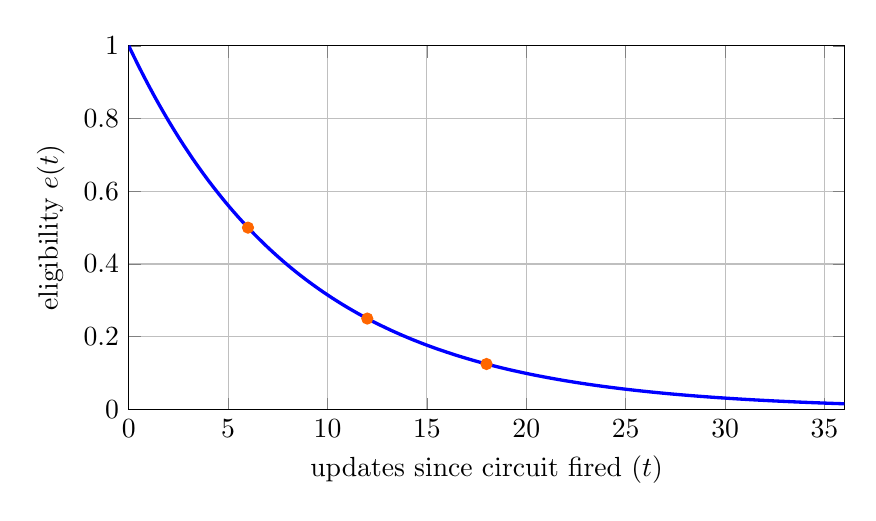
\begin{tikzpicture}
\begin{axis}[width=.88\linewidth,height=6.2cm,xlabel={updates since circuit fired ($t$)},ylabel={eligibility $e(t)$},xmin=0,xmax=36,ymin=0,ymax=1,grid=major]
\addplot[very thick,blue,domain=0:36,samples=145] {pow(0.5,x/6)};
\addplot[only marks,mark=*,red!60!yellow] coordinates {(6,.5) (12,.25) (18,.125)};
\end{axis}
\end{tikzpicture}
\caption*{\textbf{Figure 2 — Eligibility-trace decay.} The exact analytic curve of Eq. (8): \(e(t) = 0.5^{t/6}\), computed, not fitted. At the half-life \(t=6\) the trace sits at \(0.5\); at \(t=12\), \(0.25\); at \(t=18\), \(0.125\). Rewards arriving within this window reach recently firing circuits, increasingly weakly — this is the bridge between sparse feedback and the circuits that earned it.}
\end{figure}

\subsection{Weight update and reversal}

The learned weight change is the product of dopamine, trace, and learning rate, clipped to the unit box, with \(LR = 1.0\):

\begin{equation}
\Delta w = \operatorname{clip}(\mathrm{da}\cdot e\cdot LR,\; -1,\; 1), \qquad LR = 1.0
\tag{9a}
\end{equation}

\noindent\emph{Numeric example: \(\mathrm{da} = 0.40\) with a fresh trace \(e = 1.0\) yields \(\Delta w = 0.40\). If instead \(\mathrm{pe}\) is strongly negative (a punished circuit, \(\mathrm{da} = -0.50\), \(e = 1.0\)), the update is \(-0.50\) — and the \emph{reversal multiplier} fires:}

\begin{equation}
\text{on reversal:}\quad \Delta w^- = \operatorname{clip}(-1.6\,|\Delta w|,\; -1,\; 1)
\tag{9b}
\end{equation}

\noindent\emph{Negative updates are magnified by \(1.6\): unlearning a mistake is faster than learning a success. The \([-1, 1]\) clip still bounds every weight, so no sequence of updates can explode regardless of reward scale.}

This asymmetry is biologically motivated — flies forget punishment-associated odors faster than reward-associated ones — and practically motivated: on a device the user lives with, misbehaving behaviors must vanish fast and apologize rarely.

The complete per-feedback-event update is one forward pass — no backprop, no replay buffer, no gradient tape — which is what makes it auditable: diff the weights before and after a single thumbs-down and the entire credit assignment is on the table:

\begin{CodeBlock}
# Phase 10A — one feedback event through the whole update chain (reference sketch)
LR, ALPHA, HALF_LIFE = 1.0, 0.2, 6
def on_feedback(circuits, value, dopamine, reward):
    pe = reward - value["E"]                                # Eq. (6): surprise
    value["E"] = clamp(value["E"] + ALPHA * pe, -1.0, 1.0)  # Eq. (5): value estimate
    dopamine["da"] = clamp(dopamine["da"] * 0.6 + RISE * pe, -1.0, 1.0)  # Eq. (7)
    for c in circuits:
        c.trace *= 0.5 ** (1.0 / HALF_LIFE)                 # Eq. (8): half-life 6
        dw = clamp(dopamine["da"] * c.trace * LR, -1.0, 1.0)  # Eq. (9a): learned change
        if dw < 0:                                          # reversal: burn the mistake fast
            dw = clamp(-1.6 * abs(dw), -1.0, 1.0)            # Eq. (9b): reversal 1.6
        c.w = clamp(c.w + dw, -1.0, 1.0)                    # every weight stays boxed
        log_trace(name=c.name, trace=c.trace, dw=dw)        # the audit trail
\end{CodeBlock}

Phase 12 counts what this chain does: agreement that flows through this function is what \texttt{agree\_rate} measures upstream (§8.1). The update keeps the old Stage 4 numbers where they were right — delayed credit, reversal asymmetry — and replaced the parts the stages had hand-tuned with equations whose constants live in config and whose behavior a human can check against Table 2 by hand.

\section{Phase 10B: decisions to movement}

Phase 10A learns which actions were good; Phase 10B turns chosen actions into motion. It is a three-stage pipeline:

\begin{CodeBlock}
# Phase 10B configuration
AIKO_FLY_BODY_MODE=shadow
AIKO_FLY_BODY_BACKEND=null   # null | vrm | freenove
\end{CodeBlock}

\begin{enumerate}[leftmargin=*]
\item \textbf{Motor primitives} — descending-neuron-like command cells each own a small primitive (walk-to, posture, gesture, tool-grasp envelope). A decision activates primitives, not muscle torques.
\item \textbf{VNC-style coordination} — a coordinator resolves conflicts between simultaneously active primitives (two gaits cannot run at once) and sequences transitions, keeping joint/body commands coherent under load.
\item \textbf{Actuator backends} — the coordinator's command stream dispatches to a configured backend: \texttt{null} (commands logged, nothing moves — the default), \texttt{vrm} (avatar rig), or \texttt{freenove} (TCP link to the FNK0062 robot dog).
\end{enumerate}

Two operating facts matter. First, the default body backend is \texttt{null} via \texttt{AIKO\_FLY\_BODY\_BACKEND=null}: a decisions-to-movement pipeline ships with \emph{no body attached ever by default}, because driving actuators is the one modal shift that turns a software error into a physical one. Second, the giant-fiber e-stop is physical-layer, not policy-layer: the frame \texttt{F\#0\#0\#0\#} freezes the Freenove dog immediately, independent of anything the planners, voters, or LLM are doing. That e-stop is the hardware twin of the valence veto in Eq. (3) — the veto stops \emph{decisions}, the e-stop stops \emph{motion}.

\subsection{Motor primitives}

The primitive layer exported to the agent mirrors what the stages set up: Stage 6's body packet (§3.8) proved that expression/gesture/gaze could come out of DN channels, and Phase 10B formalized the downward path that can carry \emph{either that packet or plain commands}. The coordinator works on a small, fixed catalog of primitives with explicit mutual-exclusion groups (Table 15): at most eight primitives in flight at once, and no two members of an exclusion group active together — the shipped constraints the design borrowed from the connectome motif (§4.4, Table 9).

{\small
\captionof*{table}{\textbf{Table 15.} The shipped motor-primitive catalog and its arbitration groups. A request for a second member of an exclusion group aborts the running one — no blending, no queuing.}
\begin{longtable}{@{}>{\raggedright\arraybackslash}p{.22\textwidth} >{\raggedright\arraybackslash}p{.22\textwidth} >{\raggedright\arraybackslash}p{.22\textwidth} >{\raggedright\arraybackslash}p{.22\textwidth}@{}}
\toprule
\textbf{Primitive} & \textbf{Exclusion group} & \textbf{Source} & \textbf{Typical backend route} \\
\midrule
\texttt{walk-to} & gait & planner waypoint & freenove locomotion \\
\texttt{pace} & gait & drive state / exercise routine & freenove locomotion \\
\texttt{posture-sit} & posture & scheduled / idleness & freenove or vrm \\
\texttt{posture-stand} & posture & wake, alert & freenove or vrm \\
\texttt{wave} & gesture & greeting / farewell turns & vrm (avatar rig) \\
\texttt{point} & gesture & reference / instruction & vrm or null \\
\texttt{nod} & gesture & acknowledgment turns & vrm (avatar rig) \\
\texttt{tool-grasp} & manipulation & planner tool calls & freenove (gripper profile) \\
\bottomrule
\end{longtable}
}

\subsection{VNC-style coordination}

The coordinator is the one place that owns \emph{motion coherence}: it arbitrates group exclusion, orders transitions (the predecessor parks before the successor starts — no mid-pose collisions), and caps in-flight primitives. Its shape is small on purpose — conflicts resolve by priority and recency, with the loser aborted rather than queued, because a movement queue is just a delayed-motion bug with a name:

\begin{CodeBlock}
# Phase 10B — VNC-style coordination: group arbitration + transitions
EXCLUSIVE = {"gait": {"walk-to", "pace"}, "posture": {"posture-sit", "posture-stand"},
             "gesture": {"wave", "point", "nod"}, "manipulation": {"tool-grasp"}}
def coordinate(requested, active, bus):
    for group, members in EXCLUSIVE.items():
        clashing = [p for p in requested + active if p.name in members]
        if len(clashing) > 1:                       # two gaits can't run at once
            kill = min(clashing, key=lambda p: p.priority)
            yield ("abort", kill)                    # loser aborts; no queue
    for p in transition_order(requested, active):
        yield ("start_after_park", p)                # predecessor parks, then successor
\end{CodeBlock}

\subsection{Actuator backends and the e-stop}

The dispatch layer is a two-character contract with one philosophy: \emph{nothing moves unless a human configured a body}. The default \texttt{null} backend logs every would-have-moved command with its timestamp — the same log the practice world (§4.9) diffs its scenarios against — so the entire motion stack is testable with no hardware on the desk. The \texttt{vrm} backend maps packets onto the avatar rig (the same packets the Stage 6.1 endpoint in §3.9 serves), and the \texttt{freenove} backend serializes commands over TCP to the robot-dog frame protocol:

\begin{CodeBlock}
# Phase 10B — actuator backends: null is the shipped default
def dispatch(cmd):
    backend = CONF["body_backend"]                 # AIKO_FLY_BODY_BACKEND (default null)
    if backend == "null":
        motion_log.append(("null", cmd))           # logged, nothing moves — ever
        return ("null", "parked")
    if backend == "vrm":
        return vrm_rig.pose(cmd)                   # avatar rig
    if backend == "freenove":
        return tcp_send(FNK0062, cmd.frame)        # TCP link to the physical dog

def gf_estop():                                    # giant-fiber e-stop: policy-independent
    tcp_send(FNK0062, b"F#0#0#0#")                 # freeze. no state machine, no ack wait
\end{CodeBlock}

\begin{CodeBlock}
# memory.yaml (excerpt) — phase 10B movement dispatch
fly:
  body_backend: null               # null | vrm | freenove — null ships; everything else is opt-in
  freenove_tcp: 192.168.1.100:8080 # FNK0062 frame-protocol socket
  estop_frame: F#0#0#0#            # freeze frame: immediate, unconditional
  max_inflight: 8                  # coordinator cap across all primitives
\end{CodeBlock}

The two physical-layer stops line up deliberately. The \textbf{valence veto} (Eq. (3), §4.5) fires on \emph{internal} evidence — MB valence dropping below −0.6 — and acts \emph{before a decision exists}. The \textbf{e-stop} fires on receipt — a wire-level frame, no judgment, no voter — and acts \emph{after a motion has already begun}. One stops intentions; the other stops muscles. Neither is reachable by the persona machinery of §7: Eq. (3) and the e-stop are persona-blind by design, and no update to persona parameters can gate, delay, or disable them. Phase 10B closes the fly's actuation story the only honest way: \emph{one software veto, one physical freeze, and nothing in between.}

\section{Phase 11: persona-conditioned circuits}

The agent has a personality — a warm, teasing, little-sister persona — and Phase 11 lets that persona legitimately \emph{condition the circuits}: how fast urgency rises, how optimistic the value estimates are, which actions the vote weights toward. The key design decision is that persona influence is \emph{bounded and auditable}, because a personality that can quietly rewire its reflexes is indistinguishable from drift.

\begin{CodeBlock}
# Phase 11 configuration
AIKO_FLY_PERSONA_MODE=shadow
AIKO_FLY_PERSONA_LR=0.05
AIKO_FLY_PERSONA_DIR=~/.aiko/state/fly-persona
\end{CodeBlock}

Let \(\mathbf{p}\) be the persona parameter vector, \(\mathbf{p}_0\) its calibrated baseline, and \(\delta\) any single update. The shipped constraints, all enforced at write time:

\begin{equation}
|\delta| \le 0.02 \quad\text{(per update)}
\tag{10a}
\end{equation}

\begin{equation}
e_{\min} = 3\ \text{events between updates (cooldown)}
\tag{10b}
\end{equation}

\begin{equation}
|\mathbf{p} - \mathbf{p}_0| \le 0.30 \quad\text{(drift cap, per coordinate)}
\tag{10c}
\end{equation}

\noindent\emph{The step cap (10a) limits each move, the cooldown (10b) limits the move rate (at most one update per three relevant events), and the drift cap (10c) bounds the total excursion around baseline to \(\pm 0.30\). Reaching the cap takes at least \(0.30/0.02 = 15\) updates, i.e. at least \(15 \times 3 = 45\) events — a deliberate number: a persona shift you can notice from across a month, never from across an afternoon.}

Persona conditioning gates circuit \emph{gains}, never vetoes: Eq. (3) and the e-stop are persona-blind by design. Phase 11 went live in default shadow so every conditioning event could be audited against these bounds before its first live outing.

\subsection{Write-time enforcement}

The constraints above are not documented conventions — they are \emph{assertions enforced at the write site}, in the single function every persona update flows through. No update can overshoot the step cap, fire twice within one cooldown window, or drift a parameter past ±0.30 without raising, and every update — proposed or rejected — appends to a per-parameter audit trail:

\begin{CodeBlock}
# Phase 11 — persona conditioning: every update gated at write time (reference sketch)
STEP_CAP, COOLDOWN_E, DRIFT_CAP = 0.02, 3, 0.30   # Eqs. (10a), (10b), (10c)
def condition(user_id, name, delta, context):
    p = persona_params.for_user(user_id).get(name)
    audit_open(name, delta, context)              # proposed events are logged too
    if abs(delta) > STEP_CAP:                     # Eq. (10a)
        return reject(f"|delta|={abs(delta):.3f} > {STEP_CAP}")
    last = audit_log.last_applied(name)
    if context.event_index - last.event_index < COOLDOWN_E:   # Eq. (10b)
        return reject("cooldown: 3 events between updates")
    if abs(p.value + delta - p.p0) > DRIFT_CAP: # Eq. (10c)
        return reject(f"|p-p0| would exceed {DRIFT_CAP}")
    p.value += delta
    audit_log.append({"t": now(), "delta": delta, "p": p.value, "p0": p.p0,
                      "why": context.trigger, "by": context.actor})
    return accept(p.value)
\end{CodeBlock}

Because updates flow through one gate, the audit trail is the \emph{complete history of every persona parameter}: grep one name and you get its whole journey — who proposed what, why, and whether the gate let it through. The trail lives in the same format as the Phase 12 metrics (§8.1) so conditioning activity feeds the same dashboards as votes and throttle skips: persona drift is \emph{counted}, not intuited.

\subsection{What persona may — and may not — touch}

The persona vector \(\mathbf{p}\) conditions \emph{gains}: how fast urgency rises, how optimistic value estimates are, which way the action vote leans. Its knobs are the slow readouts of circuits that were themselves designed bounded (Table 16). What it \emph{cannot} touch is equally explicit: the veto path, the stopping frames, the thresholds. Vetoes are calibrated by calibration people, not felt by personalities — no persona evolution can make the agent's escape reflexes gentler.

{\small
\captionof*{table}{\textbf{Table 16.} Representative persona-conditioned gains with their calibrated baselines, plus the two stops persona can never touch.}
\begin{longtable}{@{}>{\raggedright\arraybackslash}p{.30\textwidth} >{\raggedright\arraybackslash}p{.30\textwidth} >{\raggedright\arraybackslash}p{.30\textwidth}@{}}
\toprule
\textbf{Gain} & \textbf{Baseline \(p_0\) (typical)} & \textbf{What it steers} \\
\midrule
\texttt{value\_optimism} & 0.00 & MB read-out offset; praise-laden history trends positive \\
\texttt{urgency\_rise} & 1.00 & multiplier on Phase 6 → Phase 7 salience spikes \\
\texttt{mb\_vote\_share} & 0.40 & learned-value share in the Eq. (1) vote \\
\texttt{dn\_vigor\_bias} & 1.00 & motor-economy baseline in the vote; Stage 6 packets get moodier at extremes \\
GF valence veto (−0.6) & — & \textbf{persona-blind by design:} no persona update may touch it \\
GF e-stop frame \texttt{F\#0\#0\#0\#} & — & \textbf{persona-blind by design:} no persona update may touch it \\
\bottomrule
\end{longtable}
}

Two properties complete the phase. First, persona updates are \emph{small relative to what they steer}: a ±0.30 excursion on a 0.40 vote share bends behavior (\emph{flavors} it, in the team's term) without stealing it; a −0.30 drop on the MB share is still a working vote, just less value-hungry. Second, the phase is shadow-first like everything else — Phase 11 spent its first live outing in shadow, and its audit trail was reviewed before any conditioning went live. The conditioning is \emph{mild and honest}: warmth comes from small, counted, reversible gains, not from a personality you cannot see.

\section{Phase 12: metrics + safe dial}

Eleven phases of circuits, all shadow-first, all reversible — and until Phase 12, barely visible. There was no aggregate record of what the circuits were doing, how often the expensive full-brain pass ran, or whether the dials anyone turned had any effect. Phase 12 (merged as PR \#195) is the observability-and-control capstone: a metrics module, pipeline hooks, a compute throttle, a Studio endpoint, and sane live defaults. It answers the operational question: \emph{given this device and this usage, what should the three dials be set to?}

\begin{CodeBlock}
# Phase 12 configuration
AIKO_FLY_ACTION_MODE=live
AIKO_FLY_ACTION_WEIGHT=0.25
AIKO_FULLBRAIN_EVERY_N=3
AIKO_FULLBRAIN_MIN_INTERVAL_S=2.0
\end{CodeBlock}

\begin{quote}
\small \textbf{Scope statement — read carefully.} Phase 12 is \emph{metrics + safe dial only}. It does not add leaky integrate-and-fire dynamics, it does not tune any weight automatically, and it does not change a single formula from §4–§7. The module counts what happens; \emph{humans} read the numbers and turn the dials. Any proposal to auto-tune from these metrics is a future phase, not this one.
\end{quote}

\subsection{Module: counters and \texttt{snapshot()}}

\texttt{cognition/fly\_behavior/metrics.py} holds the counters: proposed/action scores recorded, actions applied, feedback agree/disagree events, full-brain steps executed, throttle skips, and per-step wall-clock durations. \texttt{snapshot()} reduces the raw counters to the metric set served to Studio:

\begin{equation}
\mathrm{applied\_rate} = \frac{N_{\mathrm{applied}}}{N_{\mathrm{proposed}}},\qquad \mathrm{agree\_rate} = \frac{N_{\mathrm{agree}}}{N_{\mathrm{agree}} + N_{\mathrm{disagree}}}
\tag{12}
\end{equation}

\begin{equation}
\mathrm{fullbrain\_avg\_ms} = \frac{1}{N_{\mathrm{steps}}} \sum_{i=1}^{N_{\mathrm{steps}}} \mathrm{ms}_i
\tag{13}
\end{equation}

\noindent\emph{\texttt{applied\_rate} measures how often the vote's verdict is actually followed (how much the circuit output \emph{moves the agent}); \texttt{agree\_rate} measures, on recorded feedback, how often the human agreed with what happened; \texttt{fullbrain\_avg\_ms} is the mean cost of an executed full-brain step — the number against which the throttle dial is judged.}

\texttt{record\_action} / \texttt{record\_feedback} hooks sit in the action-selection and turn pipelines (\texttt{action\_select.py}, \texttt{turn.py}), so every score and every feedback event is captured exactly once. The throttle helpers live in \texttt{cognition/flymemory/fullbrain.py} and the turn wiring: \texttt{should\_step} / \texttt{mark\_stepped} / \texttt{record\_fullbrain}.

\subsection{The full-brain compute throttle}

The full-brain pass — running every circuit together for a holistic read — is the most expensive periodic computation in the stack. The Phase 12 throttle decides, on \emph{every candidate step} (at most one per turn), whether that pass runs or is deferred. It is a dual-window inequality: enough turns must have passed \emph{and} enough wall-clock time must have accumulated since the last executed step:

\begin{equation}
\text{run} \iff (\mathrm{steps\_since\_last} \ge \mathrm{EVERY\_N})\ \land\ (\mathrm{secs\_since\_last} \ge \mathrm{MIN\_INTERVAL\_S})
\tag{11}
\end{equation}

\noindent\emph{Shipped defaults: \(\mathrm{EVERY\_N} = 3\), \(\mathrm{MIN\_INTERVAL\_S} = 2.0\;\mathrm{s}\), and \texttt{AIKO\_FLY\_ACTION\_MODE=live}. Skips are counted (\texttt{fullbrain\_skipped\_throttle}) rather than silently dropped, so the ratio of skipped to executed steps is observable and becomes the dialing signal (§8.4).}

\begin{figure}[htbp]
\centering
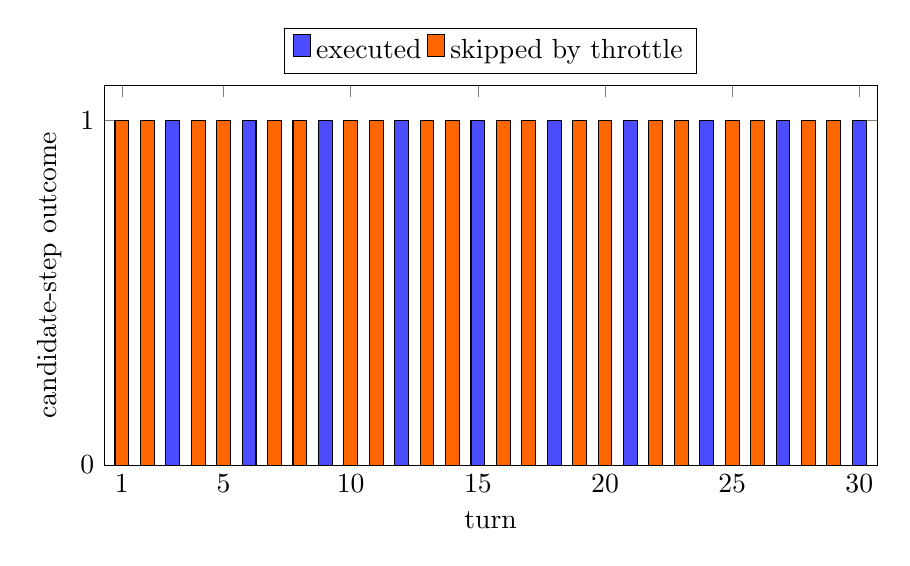
\begin{tikzpicture}
\begin{axis}[width=.94\linewidth,height=6.4cm,ybar stacked,bar width=5pt,xlabel={turn},ylabel={candidate-step outcome},xmin=.3,xmax=30.7,ymin=0,ymax=1.1,xtick={1,5,10,15,20,25,30},ytick={0,1},legend style={at={(.5,1.03)},anchor=south,legend columns=2}]
\addplot[fill=blue!70] coordinates {(1,0) (2,0) (3,1) (4,0) (5,0) (6,1) (7,0) (8,0) (9,1) (10,0) (11,0) (12,1) (13,0) (14,0) (15,1) (16,0) (17,0) (18,1) (19,0) (20,0) (21,1) (22,0) (23,0) (24,1) (25,0) (26,0) (27,1) (28,0) (29,0) (30,1)};
\addplot[fill=red!60!yellow] coordinates {(1,1) (2,1) (3,0) (4,1) (5,1) (6,0) (7,1) (8,1) (9,0) (10,1) (11,1) (12,0) (13,1) (14,1) (15,0) (16,1) (17,1) (18,0) (19,1) (20,1) (21,0) (22,1) (23,1) (24,0) (25,1) (26,1) (27,0) (28,1) (29,1) (30,0)};
\legend{executed,skipped by throttle}
\end{axis}
\end{tikzpicture}
\caption*{\textbf{Figure 3 — Throttle outcomes over 30 turns} (the illustrative session of §8.4, defaults \(\mathrm{EVERY\_N} = 3\), \(\mathrm{MIN\_INTERVAL\_S} = 2.0\;\mathrm{s}\)): bar height is one candidate step per turn; executed segments accumulate to \(10\) runs and \(20\) skips. The gap sequence between turns is fixed dataset material (§8.4), so the only free variables are the two dials.}
\end{figure}

\subsection{Studio endpoint}

\texttt{GET /studio/fly/api/metrics} (wired in \texttt{interface/webui/studio/fly/backend/api.py}) serves \texttt{snapshot()} as JSON. Below is the response for the illustrative 30-turn session whose turn-by-turn behavior is plotted in Figures 3–4:

\begin{CodeBlock}
{
  "action_scores": 128,
  "actions_applied": 81,
  "feedback_agree": 52,
  "feedback_disagree": 17,
  "applied_rate": 0.6328,
  "agree_rate": 0.7536,
  "fullbrain_steps": 10,
  "fullbrain_skipped_throttle": 20,
  "fullbrain_avg_ms": 80.8,
  "action_mode": "live",
  "throttle": {"every_n": 3, "min_interval_s": 2.0}
}
\end{CodeBlock}

Note \texttt{action\_scores > 0} (the hooks are live), nonzero \texttt{fullbrain\_steps} and \texttt{fullbrain\_skipped\_throttle} (the throttle is exercising \emph{both} branches — a throttle that only ever permits is a no-op), and rates in the sane middle. These three checks are the Phase 12 post-merge validation procedure: real conversations, then read this endpoint and confirm all three.

\subsection{Illustrative 30-turn session}

All Phase 12 charts in this report are computed from one deterministic synthetic dataset: a seeded 30-turn example conversation with fixed inter-turn gaps and seeded action/feedback sequences (the seeding makes the numbers exactly reproducible on every load). It is an \emph{illustrative example}, not a production trace — it exists to show the metrics' shape and to power the interactive simulator, and its shape is deliberately plausible rather than flattering.

\begin{quote}
\small \textbf{Data note.} The dataset (gaps, proposed/applied actions, agree/disagree events, per-step durations) is bundled into this page as literals; every number in Figures 3–4 and in the JSON sample above is computed from that one source. No number is set by hand except the seed.
\end{quote}

\begin{figure}[htbp]
\centering
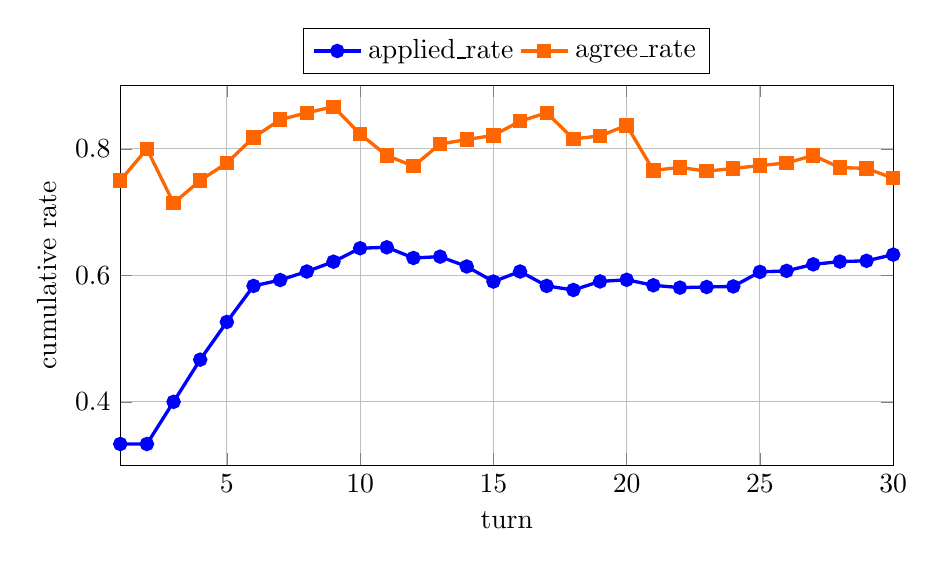
\begin{tikzpicture}
\begin{axis}[width=.94\linewidth,height=6.4cm,xlabel={turn},ylabel={cumulative rate},xmin=1,xmax=30,ymin=.3,ymax=.9,grid=major,legend style={at={(.5,1.03)},anchor=south,legend columns=2}]
\addplot[very thick,blue,mark=*] coordinates {(1,0.3333) (2,0.3333) (3,0.4000) (4,0.4667) (5,0.5263) (6,0.5833) (7,0.5926) (8,0.6061) (9,0.6216) (10,0.6429) (11,0.6444) (12,0.6275) (13,0.6296) (14,0.6140) (15,0.5902) (16,0.6061) (17,0.5833) (18,0.5769) (19,0.5904) (20,0.5930) (21,0.5843) (22,0.5806) (23,0.5816) (24,0.5825) (25,0.6055) (26,0.6071) (27,0.6174) (28,0.6218) (29,0.6230) (30,0.6328)};
\addplot[very thick,red!60!yellow,mark=square*] coordinates {(1,0.7500) (2,0.8000) (3,0.7143) (4,0.7500) (5,0.7778) (6,0.8182) (7,0.8462) (8,0.8571) (9,0.8667) (10,0.8235) (11,0.7895) (12,0.7727) (13,0.8077) (14,0.8148) (15,0.8214) (16,0.8438) (17,0.8571) (18,0.8158) (19,0.8205) (20,0.8372) (21,0.7660) (22,0.7708) (23,0.7647) (24,0.7692) (25,0.7736) (26,0.7778) (27,0.7895) (28,0.7705) (29,0.7692) (30,0.7536)};
\legend{applied\_rate,agree\_rate}
\end{axis}
\end{tikzpicture}
\caption*{\textbf{Figure 4 — Cumulative rates over the illustrative session.} \texttt{applied\_rate} rises from \(0.33\) to \(0.63\) as the warm-up circuits find their footing, ending at \(81/128 = 0.6328\); \texttt{agree\_rate} wobbles around \(0.75\)–\(0.87\), ending at \(52/69 = 0.7536\). In a healthy deployment both stay comfortably above \(0.5\); a sustained \texttt{agree\_rate} below \(0.5\) is the signal that the action mode should retreat from \texttt{live} toward \texttt{shadow} (Table 3).}
\end{figure}

\subsection{Dialing from data: the three knobs}

With the metrics visible, operating the fly stack becomes a small, explicit decision table. The order matters: \emph{cheapen first, weight second, promote last.}

{\small
\captionof*{table}{\textbf{Table 3.} The three Phase 12 dials: starting values, and the measured condition for moving each. \texttt{AIKO\_FLY\_ACTION\_WEIGHT} is the shipped \(\lambda\) of Eq. (2).}
\begin{longtable}{@{}>{\raggedright\arraybackslash}p{.30\textwidth} >{\raggedright\arraybackslash}p{.30\textwidth} >{\raggedright\arraybackslash}p{.30\textwidth}@{}}
\toprule
\textbf{Knob} & \textbf{Start} & \textbf{Move it when…} \\
\midrule
\texttt{AIKO\_FLY\_ACTION\_WEIGHT} (\(\lambda\)) & 0.25 & Raise only if \texttt{applied\_rate} is behaving usefully \emph{and} observed behavior improves under it. \\
\texttt{AIKO\_FULLBRAIN\_EVERY\_N} / \texttt{\_MIN\_INTERVAL\_S} & 3 / 2.0 & Loosen (lower) only if \texttt{fullbrain\_avg\_ms} is cheap enough that steps are affordable; raise (tighten) if the device runs hot or chat latency rises. \\
\texttt{AIKO\_FLY\_ACTION\_MODE} & live & Stay in \texttt{shadow} if disagree/veto rates look noisy; retreat live → shadow before raising any weight. \\
\bottomrule
\end{longtable}
}

The validation loop is tight on purpose: change one dial, run a few real conversations, re-read \texttt{/api/metrics}. There is no auto-tuner to blame, no hidden optimizer thread — when the weight is \(0.25\), a human put it there after looking at the numbers. That is what "safe dial" means operationally.

\section{Discussion}

\emph{What the metrics do not do.} Phase 12 exposes \texttt{applied\_rate}, \texttt{agree\_rate}, \texttt{fullbrain\_avg\_ms}, and the throttle-skip counts — and deliberately not a learning objective. A middle \texttt{applied\_rate} is not a loss to minimize; it is a \emph{temperature reading}: too low and the circuits are decoration, too high and the fly dominates the LLM it's supposed to assist. The right operating point depends on the task, the device, and observed behavior, which is why the dial stays human. Metric-driven automatic tuning is a conceivable Phase 13 — it is not this phase, and we do not pretend the shallow end of the dial is the deep end.

\emph{Why no spiking dynamics.} A leaky integrate-and-fire model would have been the biologically faithful choice for Phase 7's temporal dynamics; it was cut because the Jetson's RAM/latency budget makes spike simulation a luxury the design cannot afford, and because every circuit needs an analytic, inspectable form a human can audit from §4–§8. The bounded integrators are honest about being \emph{motifs}, not models.

\emph{The reversibility ledger.} Shadow-first deployment (§2.1) has a record now: Phase 7's shadow trail is still under review before any visual display goes live, Phase 11 spent its first live outing in shadow, and Phase 12's own post-merge procedure says to retreat to shadow before adding weight. The flags are not decoration; they are the mechanism by which a single human safely explores a neuromorphic design space on a single board computer.

\emph{Limits.} This report documents one implementation, not a family of benchmarks. Figures 3–4 are illustrative, the rate interpretations are heuristic thresholds, and the persona bounds of §7 are conservative guesses awaiting longer observation. The system's strength is corrigibility — every claim is checkable against the code, every number is bounded, and every dial points back to a person.

\section{Conclusion}

The numbered fly-brain build phases are complete: Phases 1–9 installed the reflex and habit layers, 10A added trace-based credit assignment, 10B connected decisions to movement, 11 bounded persona conditioning, and 12 (PR \#195) closed the loop with metrics and a safe dial. The circuits are small, bounded, shadow-first, and modulatory-only around an LLM core; the Phase 4 connectome is a design artifact, not a runtime load; and the operational story is now explicit: watch the meters, turn one knob at a time, retreat before you escalate. No further structural phases are required. The remaining fly work is product work — a Studio UI for the metrics and the pending Phase 7 trail review — or it is the broader roadmap beyond the fly: agents, social features, face/vision, voice.

\appendix
\section{Config flags \& phase timeline}

{\small
\captionof*{table}{\textbf{Table 4.} Key configuration constants (\texttt{config/memory.yaml} and per-phase flags). Three states apply per phase: \texttt{off}, \texttt{shadow}, \texttt{live}.}
\begin{longtable}{@{}>{\raggedright\arraybackslash}p{.30\textwidth} >{\raggedright\arraybackslash}p{.30\textwidth} >{\raggedright\arraybackslash}p{.30\textwidth}@{}}
\toprule
\textbf{Constant} & \textbf{Value} & \textbf{Effect} \\
\midrule
\texttt{AIKO\_FLY\_RUNTIME\_MODE} & off & Master switch for unverified stack passes; stays \texttt{off} on RAM-limited device until validated. \\
\texttt{AIKO\_FLY\_ACTION\_MODE} & live & Action-selection pipeline mode (Phase 12 default). \\
\texttt{AIKO\_FLY\_ACTION\_WEIGHT} (\(\lambda\)) & 0.25 & Fly share in Eq. (2)'s blend with LLM scores. \\
\texttt{AIKO\_FULLBRAIN\_EVERY\_N} & 3 & Throttle: minimum turns between full-brain steps, Eq. (11). \\
\texttt{AIKO\_FULLBRAIN\_MIN\_INTERVAL\_S} & 2.0 & Throttle: minimum seconds between full-brain steps, Eq. (11). \\
\texttt{AIKO\_FLY\_BODY\_BACKEND} & null & Movement dispatch: \texttt{null} logs without motion (default), \texttt{vrm}, or \texttt{freenove}. \\
\texttt{NIGHTLY\_PIN\_MIN\_SCORE} & 0.15 & Phase 8: minimum score for a replay pin. \\
\texttt{VETO\_VALENCE\_THRESHOLD} & −0.6 & Phase 5: giant-fiber veto of Eq. (3). \\
\bottomrule
\end{longtable}
}

\subsection{Phase timeline}

\begin{enumerate}[leftmargin=*]
\item Phase 1 — Watchdog --- live --- Whole-box RSS visibility and timeout-protected busy gate.
\item Phase 2 — Effort gating --- live --- Deduplicated embeddings/dopamine, singleton FlyDN, batched writes.
\item Phase 3 — Routine tidying --- live --- Lazy voice boot, one scheduler, ledger retention, slower background cadence.
\item Phase 4 — Connectome reference --- runtime --- 166,606-neuron / 25,574,615-edge two-hop MaleCNS rate runtime.
\item Phase 5 — Action voting --- live --- MB/CX/DN/GF vote \((0.40,0.20,0.20,0.20)\); \(\lambda=0.25\) blend; \(-0.6\) veto.
\item Phase 6 — Tone/movement listening --- live --- Pre-semantic tone and motion-energy listeners on fast paths.
\item Phase 7 — Bounded temporal dynamics --- live --- Heading/urgency/drive integrators; Studio trail still under review before display.
\item Phase 8 — Nightly replay --- live --- Idempotent nightly consolidation with min-score floor \(0.15\).
\item Phase 9 — Practice world --- live --- Sandboxed play against stubbed \texttt{null} actuators.
\item Phase 10A — Delayed credit assignment --- live --- Eligibility traces (half-life 6), \(\alpha=0.2\) value updates, dopamine × reversal 1.6.
\item Phase 10B — Decisions to movement --- live --- DN primitives → coordination → \texttt{null}/\texttt{vrm}/\texttt{freenove}; GF e-stop \texttt{F\#0\#0\#0\#}.
\item Phase 11 — Persona conditioning --- live --- Persona gain bounds \(|\delta|\le 0.02\), 3-event cooldown, \(\pm 0.30\) drift cap.
\item Phase 12 — Metrics + safe dial --- live --- Metrics module, throttle, \texttt{GET /studio/fly/api/metrics}; merged PR \#195 (2026-09-30).
\end{enumerate}

The timeline counter runs to thirteen list positions because Phase 10 split into two sub-phases (10A, 10B): twelve named phases total. Phase 12's merge closed the numbered build sequence.

\section*{References}
\addcontentsline{toc}{section}{References}

\begin{enumerate}[leftmargin=*]
\item Berg, S., Beckett, I. R., Costa, M., Schlegel, P., Januszewski, M., Marin, E. C., Nern, A., et al. (2026). \emph{Sexual dimorphism in the complete connectome of the Drosophila male central nervous system.} Cell 189, 5504–5526.e15. MaleCNS v1.0 data, CC BY 4.0; preprint bioRxiv 2025.10.09.680999.
\item Aiko-chan Project. (2026). \emph{Fly-brain wiring migration; active MaleCNS runtime; Stages 1-6.1; Fly stack complete; Phase 12 metrics + safe dial.} Repository documentation snapshot, 30 September 2026.
\item Aiko-chan Project. (2026). Phase implementation commits: guard the box (8eeefa2), stop the waste (003493d), quiet headless (eb471bc), full MaleCNS (e7da120), action selection (b04e184), sensory pathways (808f2aa), CX dynamics (4be0d2e), replay (73dbba6), FlyWorld (402baae), delayed credit (55f243f), motor circuits (f958209), persona (347108b), and metrics (2194fed / merged PR \#195).
\end{enumerate}

Fly-Brain Circuits for a Personal AI Agent · Aiko-chan project technical report · 30 September 2026.\textbf{Fly-Brain Circuits for a Personal AI Agent} · Aiko-chan project technical report, 30 September 2026.

Code excerpts are abridged for exposition; numeric constants and file-level claims are grounded in the repository snapshot cited above.

\end{document}
